\documentclass[conference]{IEEEtran}

% =========================
% PACKAGE
% =========================
\usepackage[utf8]{inputenc}
\usepackage{cite}
\usepackage{amsmath,amssymb,amsfonts}
\usepackage{graphicx}
\usepackage{textcomp}
\usepackage{xcolor}
\usepackage{float}
\usepackage{caption}
\usepackage{afterpage}
\usepackage{pdfpages}
\usepackage{verbatim}
\usepackage{listings}

\begin{document}

% ==========================================================
% HALAMAN COVER (BERDASARKAN COVER.DOCX)
% ==========================================================
\begin{titlepage}
\onecolumn
\centering
\thispagestyle{empty}

\vspace*{0.5cm}

{\fontsize{16pt}{22pt}\selectfont\bfseries LAPORAN PROGRESS\par}
\vspace{0.4cm}
{\fontsize{14pt}{18pt}\selectfont\bfseries Mata Kuliah Workshop Pemrograman Framework\par}
\vspace{0.3cm}
{\fontsize{14pt}{18pt}\selectfont\bfseries Dokumen PRD\par}

\vfill


\includegraphics[width=7.5cm]{pens_logo.png}\par

\vfill

{\fontsize{12pt}{16pt}\selectfont\bfseries Dosen Pengampu:\par}
\vspace{0.2cm}
{\fontsize{12pt}{16pt}\selectfont Amma Liesvarastranta Haz, S.Tr.T., M.T.\par}

\vspace{0.8cm}

{\fontsize{12pt}{16pt}\selectfont\bfseries Disusun Oleh:\par}
\vspace{0.25cm}
{\fontsize{12pt}{16pt}\selectfont 1. Ahmad Falihul Hikam (3125521007)\par}
\vspace{0.15cm}
{\fontsize{12pt}{16pt}\selectfont 2. Arvin Dzaky Nugraha (3125521027)\par}

\vfill

{\fontsize{13pt}{18pt}\selectfont\bfseries PROGRAM STUDI D3 TEKNIK INFORMATIKA\par}
\vspace{0.15cm}
{\fontsize{13pt}{18pt}\selectfont\bfseries DEPARTEMEN TEKNIK INFORMATIKA DAN KOMPUTER\par}
\vspace{0.15cm}
{\fontsize{13pt}{18pt}\selectfont\bfseries POLITEKNIK ELEKTRONIKA NEGERI SURABAYA\par}
\vspace{0.2cm}
{\fontsize{13pt}{18pt}\selectfont\bfseries 2026\par}

\vspace*{0.5cm}
\end{titlepage}

\clearpage
\twocolumn

\title{SIGAP: Sistem Informasi Pengaduan Perundungan dan Kekerasan Pelajar Berbasis Platform Digital dan Kecerdasan Buatan}

\maketitle

\noindent\textbf{Abstract---}
\textbf{Perundungan (\textit{bullying}) dan \textit{cyberbullying} di lingkungan pendidikan memerlukan saluran pelaporan yang aman, terstruktur, dan akuntabel. Penelitian ini mengembangkan SIGAP (Sistem Informasi Pengaduan Perundungan dan Kekerasan Pelajar), platform digital terpadu dengan pelaporan anonim maupun teridentifikasi, penjejakan tiket (\textit{ticket tracking}), serta jejak audit (\textit{audit trail}). SIGAP mengintegrasikan pemrosesan bahasa alami (\textit{Natural Language Processing}/NLP) berbasis \textit{embedding} Bahasa Indonesia untuk rekomendasi kategori dan klasterisasi laporan serupa guna mendukung pengambilan keputusan admin. Keandalan sistem diuji melalui kerangka metode validasi komprehensif, meliputi validasi teknis logika dan transisi status (\textit{state transition}), \textit{User Acceptance Testing} (UAT), \textit{System Usability Scale} (SUS), evaluasi berbasis tugas (\textit{Task Success Rate} dan \textit{Single Ease Question}/SEQ), serta validasi kualitas model AI. Karena proses evaluasi berada pada tahap pra-iterasi pengujian pengguna, parameter capaian dipetakan menggunakan metrik dasar dengan target pemenuhan skenario UAT pelapor dan admin sebesar [xx/yy], skor \textit{usability} SUS siswa [xx/100] dan admin [xx/100] (target benchmark $>$ 68), \textit{Task Success Rate} alur pelaporan siswa sebesar [xx/yy] dengan SEQ [xx/7], \textit{Task Success Rate} verifikasi admin sebesar [xx/yy] dengan SEQ [xx/7], serta akurasi klasifikasi model AI sebesar [xx\%]. Kerangka validasi ini memastikan SIGAP siap diimplementasikan secara teruji, andal, dan efektif dalam pengelolaan laporan perundungan di sekolah.}

\vspace{0.5em}

\noindent\textbf{Index Terms---}
Cyberbullying, Perundungan Pelajar, SIGAP, Sistem Pengaduan, Kecerdasan Buatan, Natural Language Processing.

\section{INTRODUCTION}

Perkembangan teknologi informasi dan komunikasi telah memberikan berbagai kemudahan dalam kehidupan masyarakat, termasuk dalam bidang pendidikan. Namun, perkembangan tersebut juga menimbulkan tantangan baru berupa munculnya tindakan perundungan melalui media digital atau \textit{cyberbullying}. \textit{Cyberbullying} merupakan bentuk perundungan yang dilakukan dengan memanfaatkan teknologi informasi dan komunikasi, seperti media sosial, pesan elektronik, dan berbagai platform digital lainnya. Zhang et al. menjelaskan bahwa perkembangan media sosial dan teknologi berbasis internet menyebabkan masyarakat semakin terhubung, tetapi pada saat yang sama menciptakan ruang baru bagi terjadinya perilaku perundungan terhadap anak dan remaja \cite{zhang2022}.

Permasalahan tersebut menjadi semakin penting karena anak dan remaja merupakan kelompok yang aktif menggunakan internet dan media sosial. Penelitian Amanatin dan Sekarningrum menunjukkan bahwa \textit{cyberbullying} pada remaja telah menjadi persoalan di beberapa wilayah perkotaan Indonesia, termasuk Jakarta, Bandung, dan Surabaya. Penelitian tersebut mengidentifikasi berbagai bentuk dan penyebab \textit{cyberbullying} yang terjadi pada remaja dalam konteks lingkungan perkotaan Indonesia \cite{amanatin2024}. Hal tersebut menunjukkan bahwa permasalahan perundungan digital tidak hanya menjadi isu global, tetapi juga memiliki relevansi yang kuat dalam lingkungan pendidikan di Indonesia.

Lingkungan sekolah juga memiliki peran penting dalam munculnya maupun pencegahan perilaku \textit{cyberbullying}. Maftuh et al. melakukan penelitian terhadap 384 siswa SMA dari enam sekolah negeri dan swasta di Magelang dan menemukan bahwa perilaku \textit{cyberbullying} berkaitan dengan kondisi iklim sekolah serta \textit{psychological capital} siswa. Penelitian tersebut juga menunjukkan bahwa penggunaan media sosial dapat memengaruhi hubungan antara faktor lingkungan sekolah dan perilaku \textit{cyberbullying} \cite{maftuh2024}. Dengan demikian, penanganan perundungan tidak cukup hanya berfokus pada pelaku dan korban, tetapi juga membutuhkan lingkungan sekolah yang mampu mendukung proses pelaporan, pencegahan, dan penanganan kasus secara sistematis.

Dampak perundungan terhadap siswa juga perlu menjadi perhatian serius. Li et al. melalui meta-analisis terhadap 42 penelitian dengan total 266.888 partisipan menunjukkan bahwa \textit{bullying} tradisional dan \textit{cyberbullying} memiliki hubungan dengan berbagai permasalahan psikologis pada anak dan remaja \cite{li2024}. Temuan tersebut memperlihatkan bahwa perundungan bukan sekadar permasalahan sosial di lingkungan sekolah, tetapi dapat berkaitan dengan kondisi psikologis dan kesejahteraan siswa. Oleh karena itu, diperlukan mekanisme penanganan yang dapat membantu pihak sekolah menerima informasi mengenai kejadian perundungan secara lebih terstruktur.

Permasalahan lainnya adalah bagaimana kasus perundungan dapat dilaporkan dan dikelola secara efektif. Dalam lingkungan sekolah, siswa yang mengalami atau mengetahui suatu kejadian perundungan memerlukan saluran pelaporan yang mudah digunakan dan mampu memberikan rasa aman. Sistem pelaporan juga perlu mampu menangani berbagai bentuk perundungan, baik perundungan verbal, fisik, sosial, maupun \textit{cyberbullying}. Evangelio et al. melalui systematic review mengenai \textit{cyberbullying} pada siswa sekolah dasar dan menengah menunjukkan bahwa program pencegahan \textit{cyberbullying} dapat memberikan hasil yang efektif, termasuk ketika pencegahan dilakukan sejak usia sekolah \cite{evangelio2022}. Upaya preventif di kalangan siswa juga menjadi bagian penting dalam membangun kesadaran dan perlindungan terhadap perundungan dunia maya \cite{eleanora2021}.

Selain menyediakan mekanisme pelaporan, sistem digital perlu memiliki kemampuan untuk membantu pihak sekolah mengelola informasi yang masuk. Jumlah laporan yang semakin banyak dapat membuat proses identifikasi dan pengelompokan kasus menjadi lebih kompleks apabila dilakukan sepenuhnya secara manual. Dalam konteks ini, teknologi kecerdasan buatan dapat digunakan sebagai alat bantu pengambilan keputusan, bukan sebagai pengganti keputusan pihak sekolah. Berdasarkan kajian Kasturiratna et al., yang mencakup 56 meta-analisis dan 296 \textit{effect sizes}, \textit{cyberbullying} memiliki berbagai faktor risiko, konsekuensi psikologis dan perilaku, serta membutuhkan intervensi yang tepat untuk mengurangi dampaknya \cite{kasturiratna2025}.

Penggunaan teknologi untuk membantu proses identifikasi juga perlu memperhatikan konsistensi dalam mendefinisikan dan mengklasifikasikan \textit{cyberbullying}. Zhang et al. menunjukkan bahwa penelitian mengenai \textit{cyberbullying} telah menggunakan berbagai definisi dan instrumen pengukuran, sehingga pemilihan kategori dan metode identifikasi perlu dilakukan secara hati-hati \cite{zhang2022}. Oleh karena itu, pemanfaatan model pemrosesan bahasa alami (\textit{Natural Language Processing}/NLP) dapat menjadi salah satu pendekatan untuk membantu menganalisis isi laporan yang ditulis oleh siswa. Dalam rancangan SIGAP, pendekatan tersebut dapat digunakan untuk menghasilkan rekomendasi kategori laporan berdasarkan isi pengaduan, sedangkan keputusan akhir tetap berada pada pihak admin atau petugas yang berwenang.

Berdasarkan permasalahan tersebut, diperlukan sebuah sistem yang tidak hanya berfungsi sebagai media pengaduan, tetapi juga mampu mendukung proses pengelolaan dan tindak lanjut laporan secara terstruktur. SIGAP (Sistem Informasi Pengaduan Perundungan dan Kekerasan Pelajar) dirancang sebagai platform digital yang memungkinkan siswa menyampaikan laporan mengenai perundungan atau kekerasan, baik secara anonim maupun dengan identitas, memperoleh tiket pengaduan, serta memantau perkembangan laporan. Pada sisi pengelola, sistem menyediakan fitur verifikasi, pengelompokan laporan, rekomendasi kategori berbasis AI, pemantauan status, serta pencatatan aktivitas (\textit{audit trail}). Pendekatan tersebut diharapkan dapat membantu menciptakan proses pelaporan yang lebih terstruktur, terdokumentasi, dan mudah dipantau.

Dengan demikian, SIGAP diharapkan dapat menjadi salah satu pendekatan teknologi dalam mendukung proses pelaporan dan penanganan perundungan di lingkungan pendidikan. Sistem ini tidak dimaksudkan untuk menggantikan peran guru, konselor, atau pihak sekolah dalam mengambil keputusan, tetapi sebagai sarana pendukung agar informasi pengaduan dapat diterima, dikategorikan, diverifikasi, dan ditindaklanjuti secara lebih sistematis. Hal ini sejalan dengan temuan penelitian yang menunjukkan pentingnya intervensi dan dukungan lingkungan dalam menangani \textit{cyberbullying} serta perlunya pendekatan yang lebih terstruktur untuk melindungi siswa \cite{maftuh2024,kasturiratna2025}.

\begin{thebibliography}{00}

\bibitem{zhang2022}
W. Zhang, S. Huang, L. Lam, R. Evans, and C. Zhu, ``Cyberbullying definitions and measurements in children and adolescents: Summarizing 20 years of global efforts,'' \textit{Frontiers in Public Health}, vol. 10, 2022, Art. no. 1000504, doi: 10.3389/fpubh.2022.1000504.

\bibitem{amanatin2024}
E. L. Amanatin and B. Sekarningrum, ``Causes and Forms of Cyberbullying among Teenagers in Indonesian Urban Areas: Cases of Jakarta, Bandung and Surabaya,'' \textit{JISPO Jurnal Ilmu Sosial dan Ilmu Politik}, vol. 13, no. 2, pp. 233--254, 2024, doi: 10.15575/jispo.v13i2.27792.

\bibitem{maftuh2024}
B. Maftuh, A. Dahliyana, E. Malihah, and R. Sartika, ``Does school climate matter in cyberbullying behaviour among high school student? A mediation and moderation analysis,'' \textit{Jurnal Cakrawala Pendidikan}, vol. 43, no. 1, pp. 28--43, 2024, doi: 10.21831/cp.v43i1.65213.

\bibitem{li2024}
C. Li, P. Wang, M. Martin-Moratinos, M. Bella-Fernández, and H. Blasco-Fontecilla, ``Traditional bullying and cyberbullying in the digital age and its associated mental health problems in children and adolescents: A meta-analysis,'' \textit{European Child \& Adolescent Psychiatry}, vol. 33, pp. 2895--2909, 2024, doi: 10.1007/s00787-022-02128-x.

\bibitem{evangelio2022}
C. Evangelio, P. Rodríguez-González, J. Fernández-Río, and S. Gonzalez-Villora, ``Cyberbullying in elementary and middle school students: A systematic review,'' \textit{Computers \& Education}, vol. 176, 2022, Art. no. 104356, doi: 10.1016/j.compedu.2021.104356.

\bibitem{kasturiratna2025}
K. T. A. S. Kasturiratna, A. Hartanto, C. H. Y. Chen, E. M. W. Tong, et al., ``Umbrella review of meta-analyses on the risk factors, protective factors, consequences and interventions of cyberbullying victimization,'' \textit{Nature Human Behaviour}, vol. 9, pp. 101--132, 2025, doi: 10.1038/s41562-024-02011-6.

\bibitem{eleanora2021}
F. N. Eleanora and R. A. Al Adawiah, ``Perundungan dunia maya (Cyberbullying) dan upaya preventif di kalangan siswa SMK Bangun Persada Bekasi,'' \textit{Jurnal Abdi Masyarakat Indonesia}, vol. 1, no. 2, pp. 203--208, 2021, doi: 10.54082/jamsi.67.

\end{thebibliography}

% ===== Mulai bagian non-IEEE: satu kolom, tanpa nomor halaman =====
\clearpage
\onecolumn
\pagestyle{empty}

\begin{center}
	{\Large\bfseries II. SOURCE CODE}\par
\end{center}

\lstinputlisting[
	language={[LaTeX]TeX},
	basicstyle=\ttfamily\footnotesize,
	breaklines=true,
	breakatwhitespace=false,
	columns=fullflexible,
	keepspaces=true,
	literate={é}{{\'e}}1 {ó}{{\'o}}1 {á}{{\'a}}1 {í}{{\'i}}1,
	frame=single,
	framerule=0.3pt,
	rulecolor=\color{black!35},
	xleftmargin=1cm,
	xrightmargin=1cm,
	framexleftmargin=4pt,
	framexrightmargin=4pt
]{SIGAP-source.tex}

\clearpage
\begin{center}
	{\Large\bfseries III. ARSITEKTUR SISTEM}\par
\end{center}

Arsitektur SIGAP mengintegrasikan lapisan \textit{User Client}, \textit{Backend Services}, \textit{AI Pipeline}, dan \textit{External Data}. Pengguna (siswa dan admin/guru BK) berinteraksi melalui antarmuka berbasis REST API/HTTPS (didukung autentikasi JWT) serta \textit{WebSocket Gateway} untuk pembaruan status dan notifikasi secara \textit{real-time}. Layanan backend FastAPI mengelola basis data relasional MySQL dan \textit{Local File Storage} untuk berkas bukti pengaduan. Teks deskripsi laporan diproses oleh \textit{AI Pipeline} berbasis IndoBERT \textit{Embedding} yang bercabang ke \textit{Cosine Similarity} (menghasilkan rekomendasi kategori dan skor keyakinan) serta HDBSCAN (mengelompokkan klaster laporan serupa). Hasil AI berstatus \textit{pending review} sebagai pendukung keputusan admin dalam menetapkan kategori final. Setiap validasi dan perubahan status dicatat pada \textit{Audit Trail}, sedangkan data eksternal (Satu Data Indonesia, SIMFONI PPA) dimanfaatkan sebagai \textit{one-time seed/training} pada inisialisasi model.

\begin{figure}[H]
	\centering
	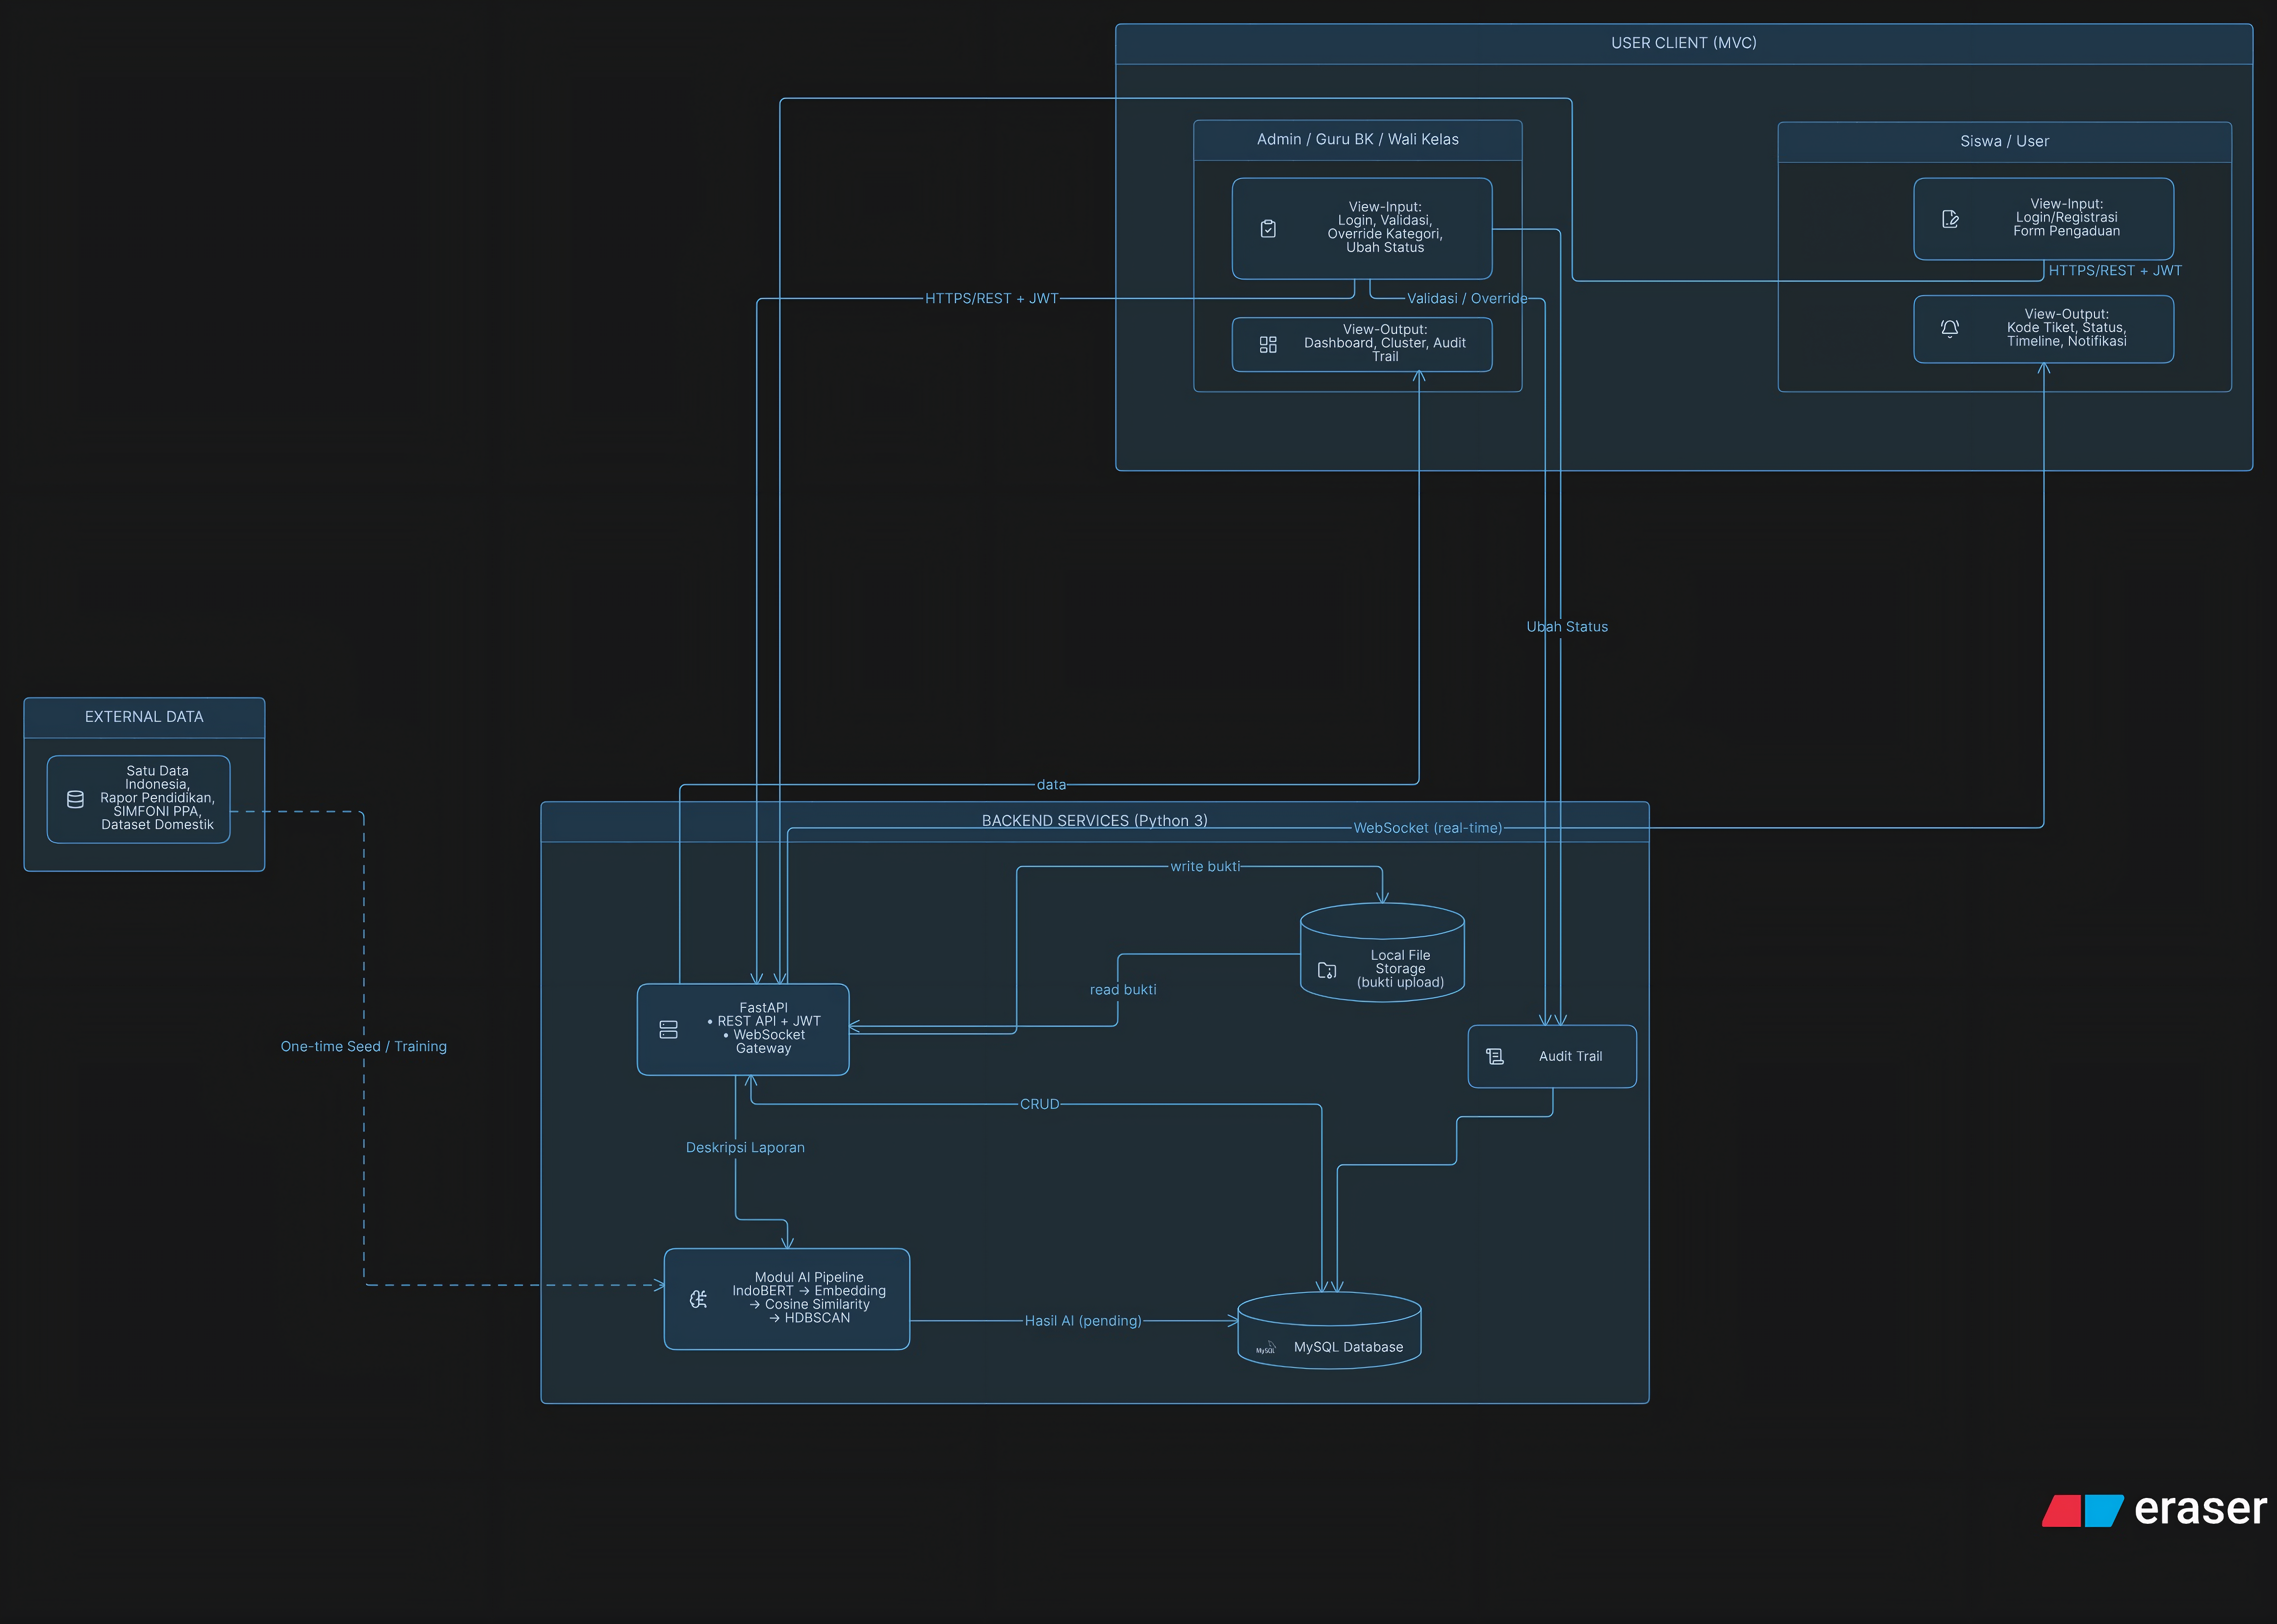
\includegraphics[width=\linewidth,height=0.62\textheight,keepaspectratio]{New_Arsitektur_Sistem.png}
	\caption{Arsitektur Sistem SIGAP}
	\label{fig:arsitektur-sigap}
\end{figure}

\clearpage
\begin{center}
	{\Large\bfseries IV. DESAIN SISTEM}\par
\end{center}

\begin{figure}[H]
	\centering
	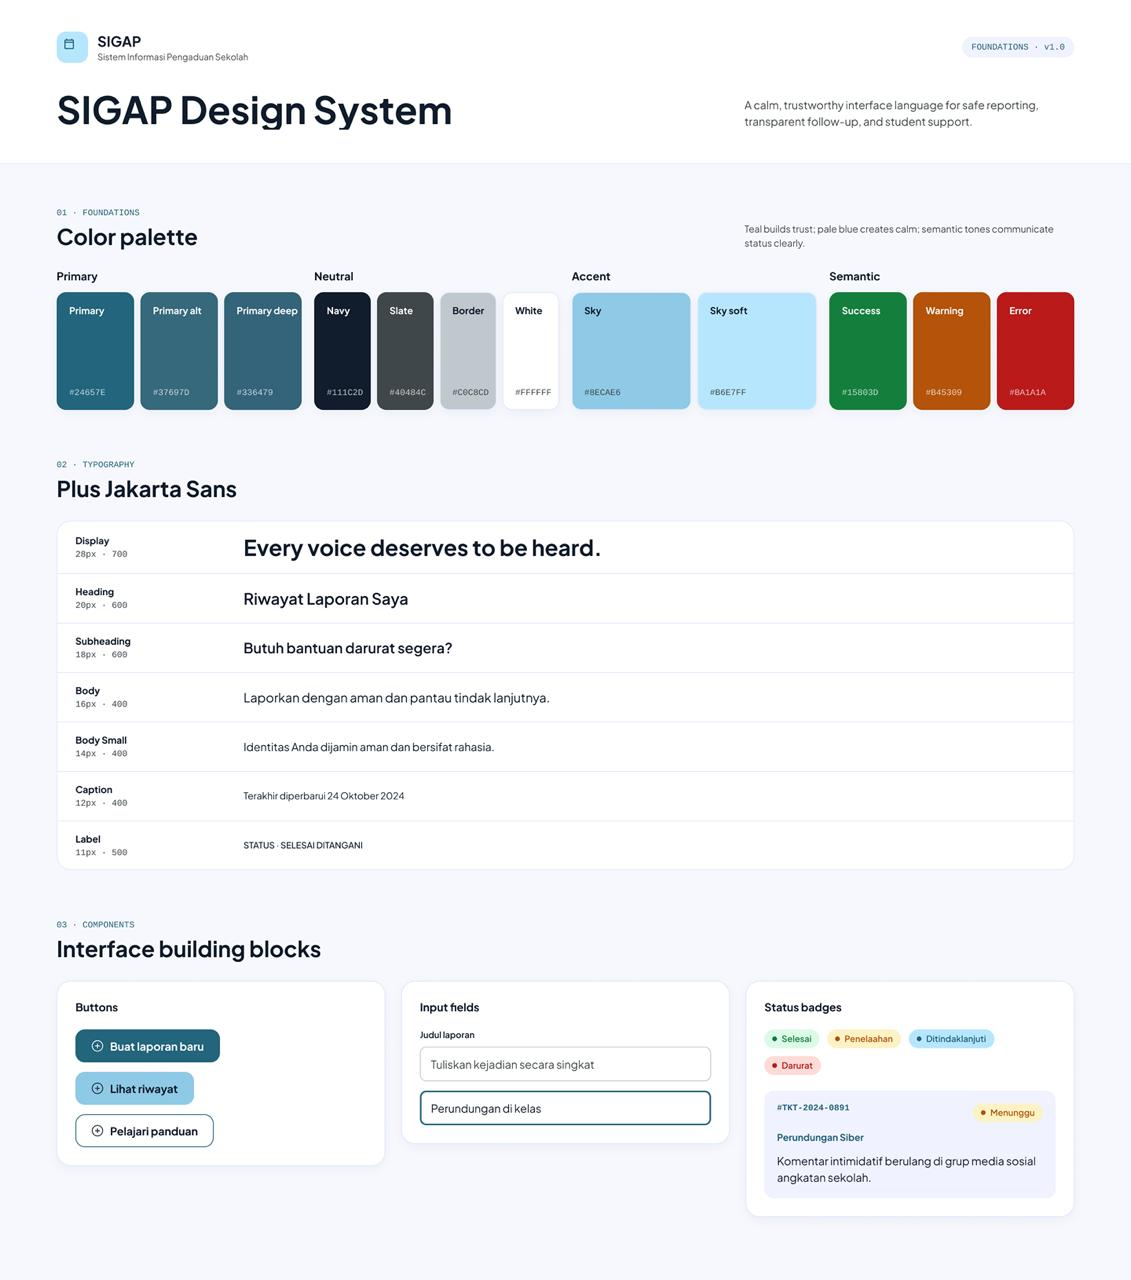
\includegraphics[width=\linewidth,height=0.72\textheight,keepaspectratio]{Desain Sistem/DesainSistem_SIGAP.png}
	\caption{Desain Sistem SIGAP}
	\label{fig:desain-sigap}
\end{figure}

\clearpage
\begin{center}
	{\Large\bfseries V. MOCKUP UI}\par
\end{center}

% --- 2 gambar per baris ---
\noindent
\begin{minipage}[t]{0.48\linewidth}
	\centering
	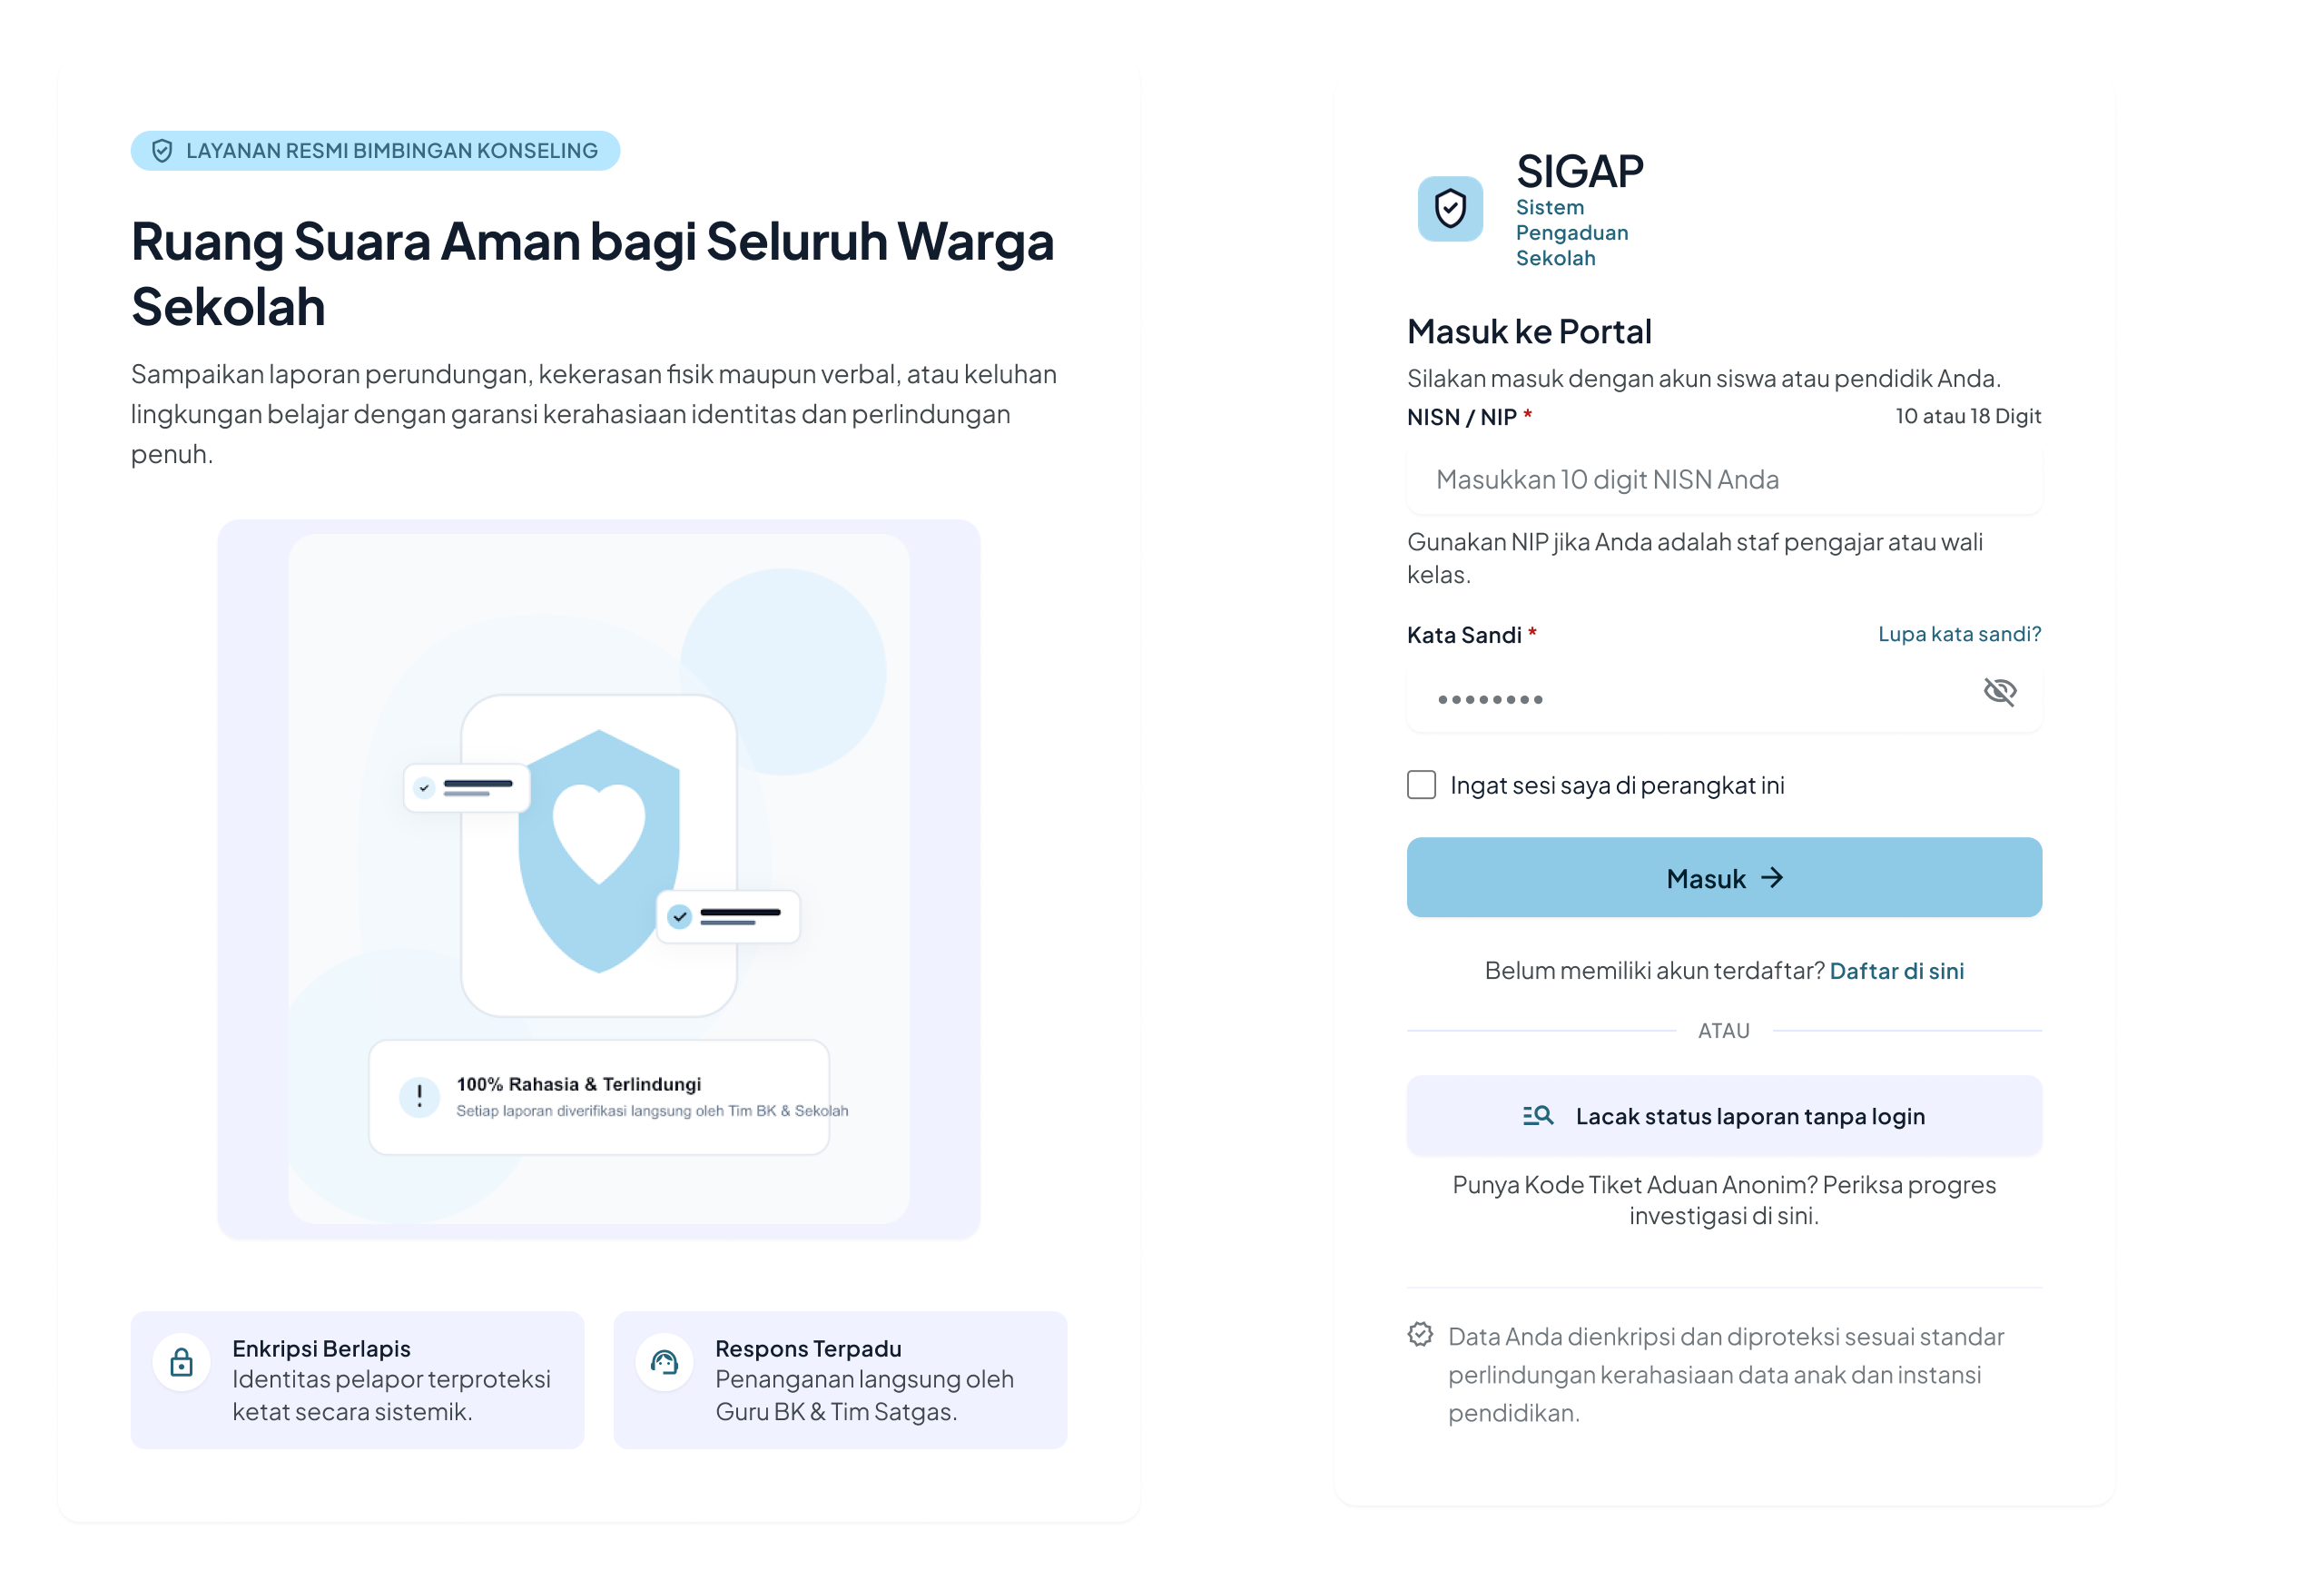
\includegraphics[width=\linewidth,height=0.42\textheight,keepaspectratio]{Frontend_image/OnBoardingUser_SIGAP.png}
	\captionof{figure}{Onboarding pengguna siswa}
\end{minipage}
\hfill
\begin{minipage}[t]{0.48\linewidth}
	\centering
	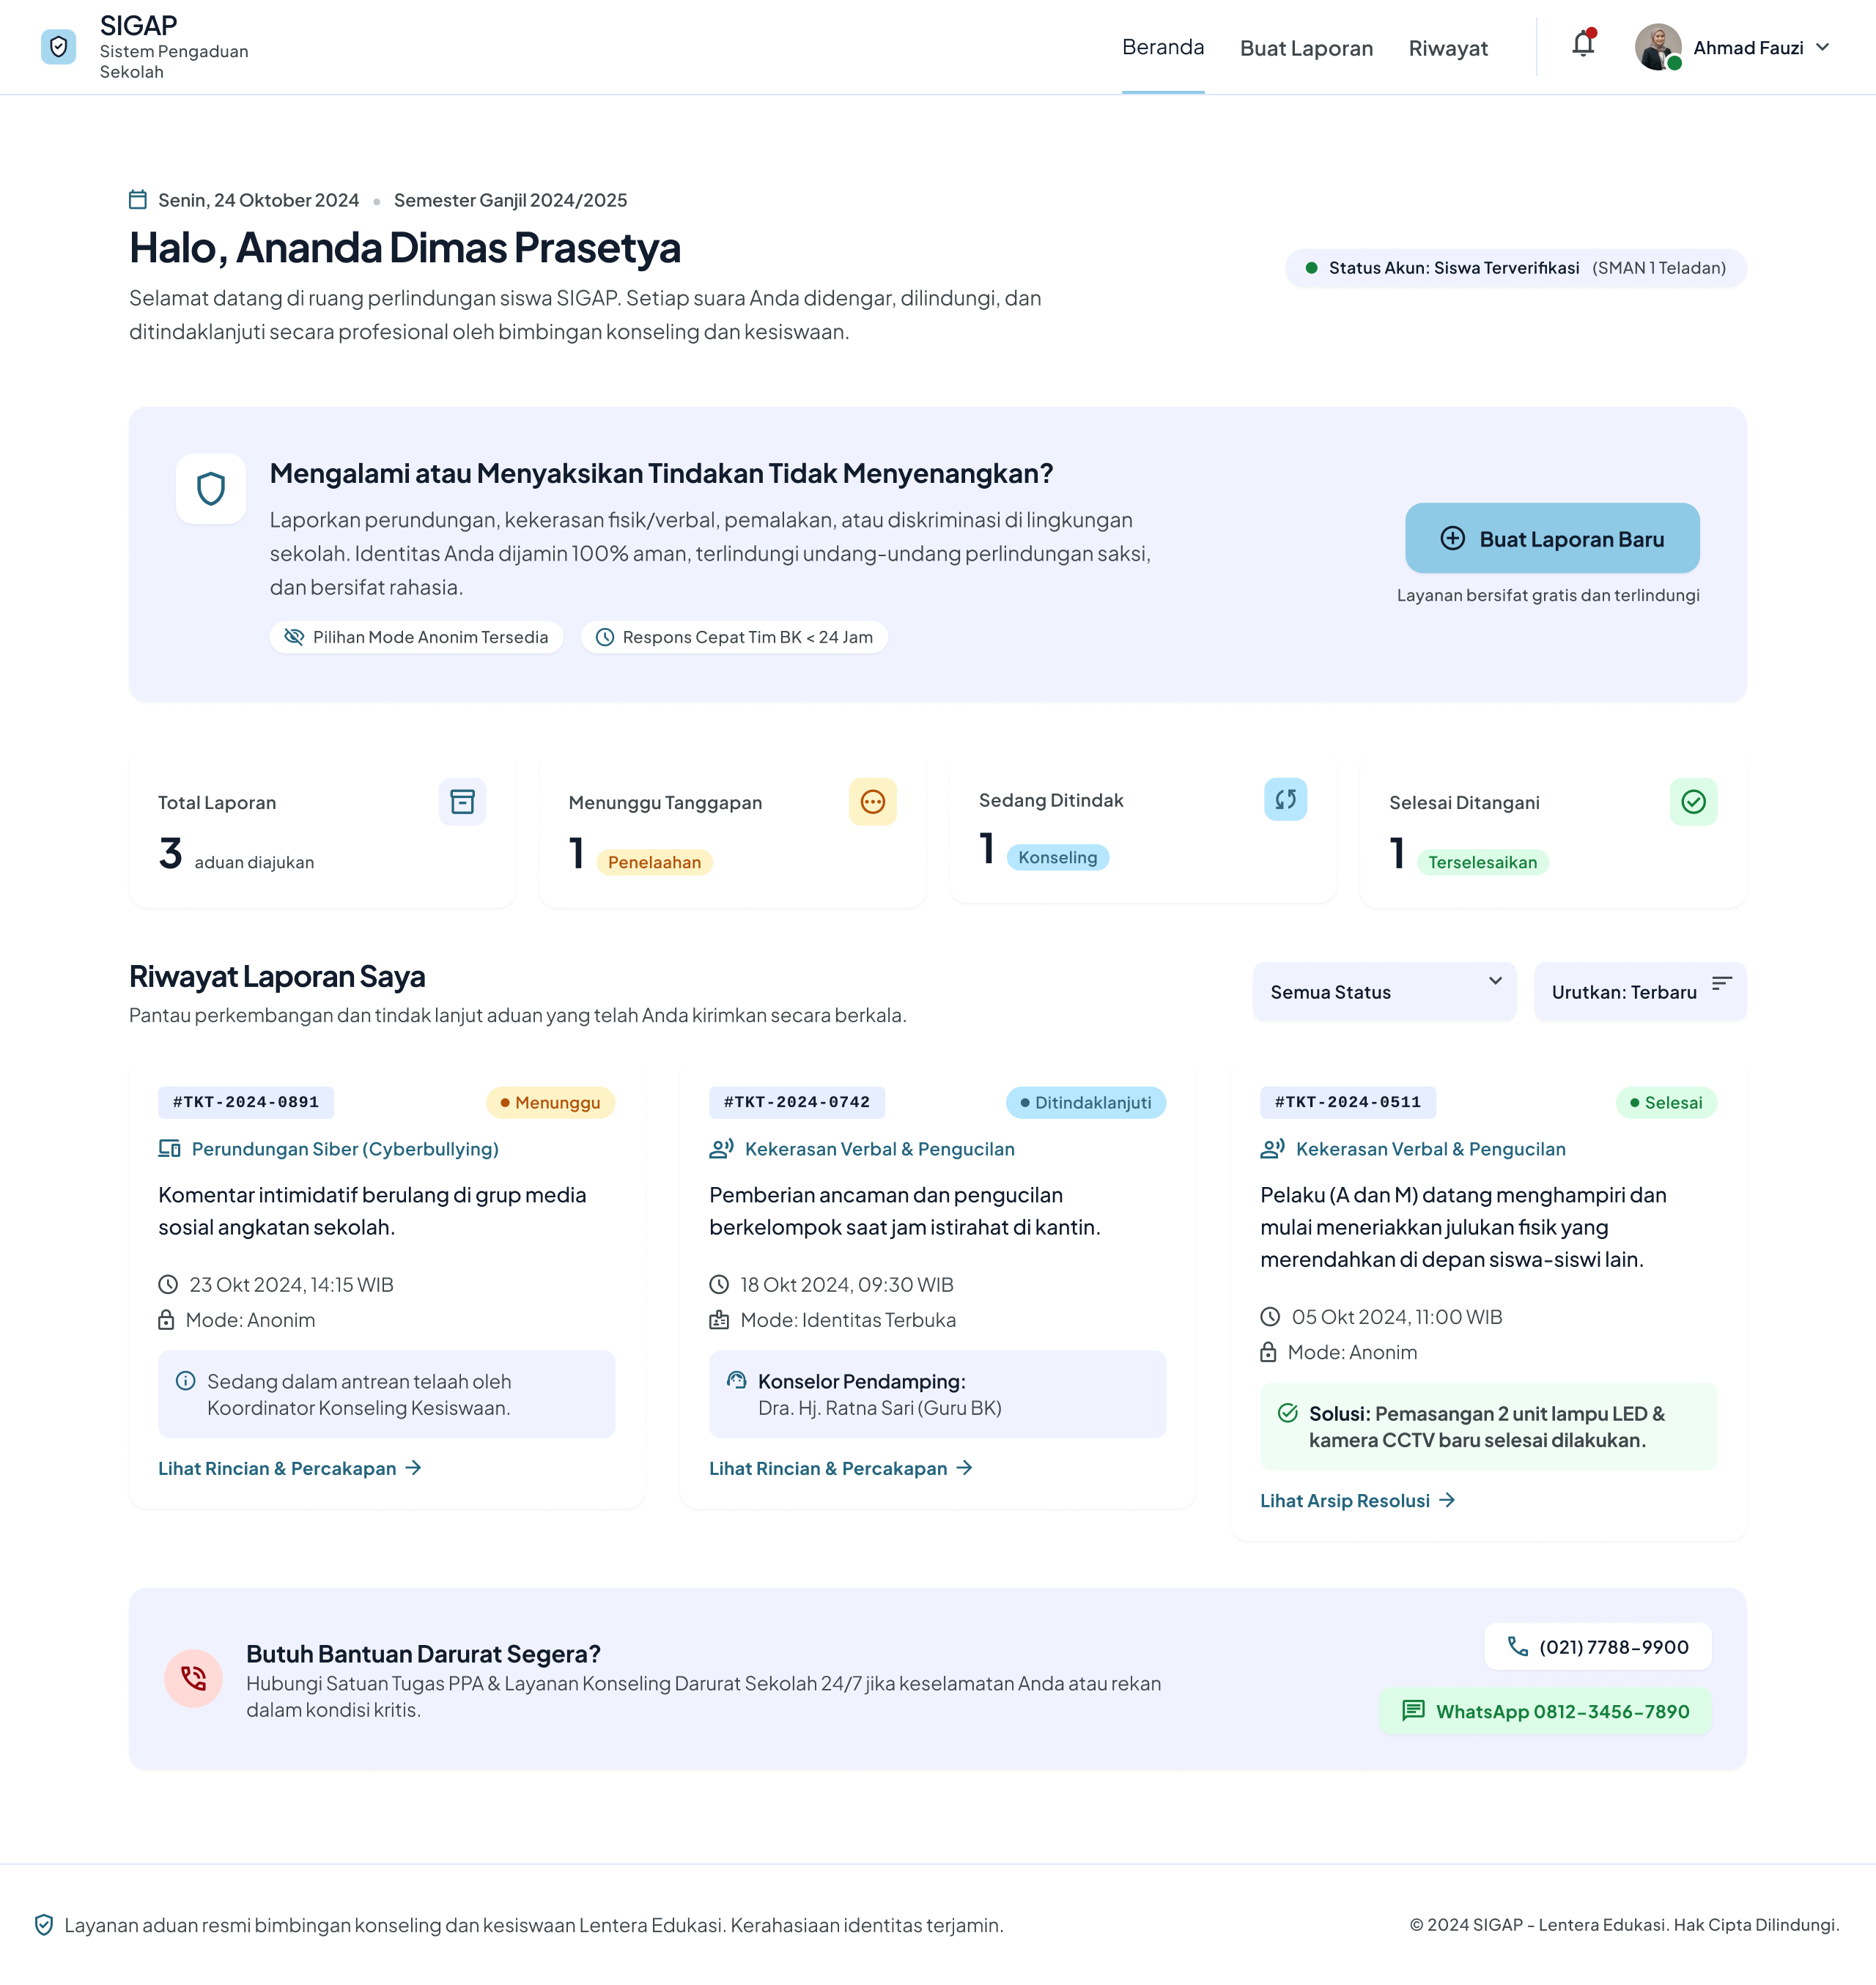
\includegraphics[width=\linewidth,height=0.42\textheight,keepaspectratio]{Frontend_image/DashboardUser_SIGAP.png}
	\captionof{figure}{Dashboard pengguna siswa}
\end{minipage}

\vspace{0.8cm}
\noindent
\begin{minipage}[t]{0.48\linewidth}
	\centering
	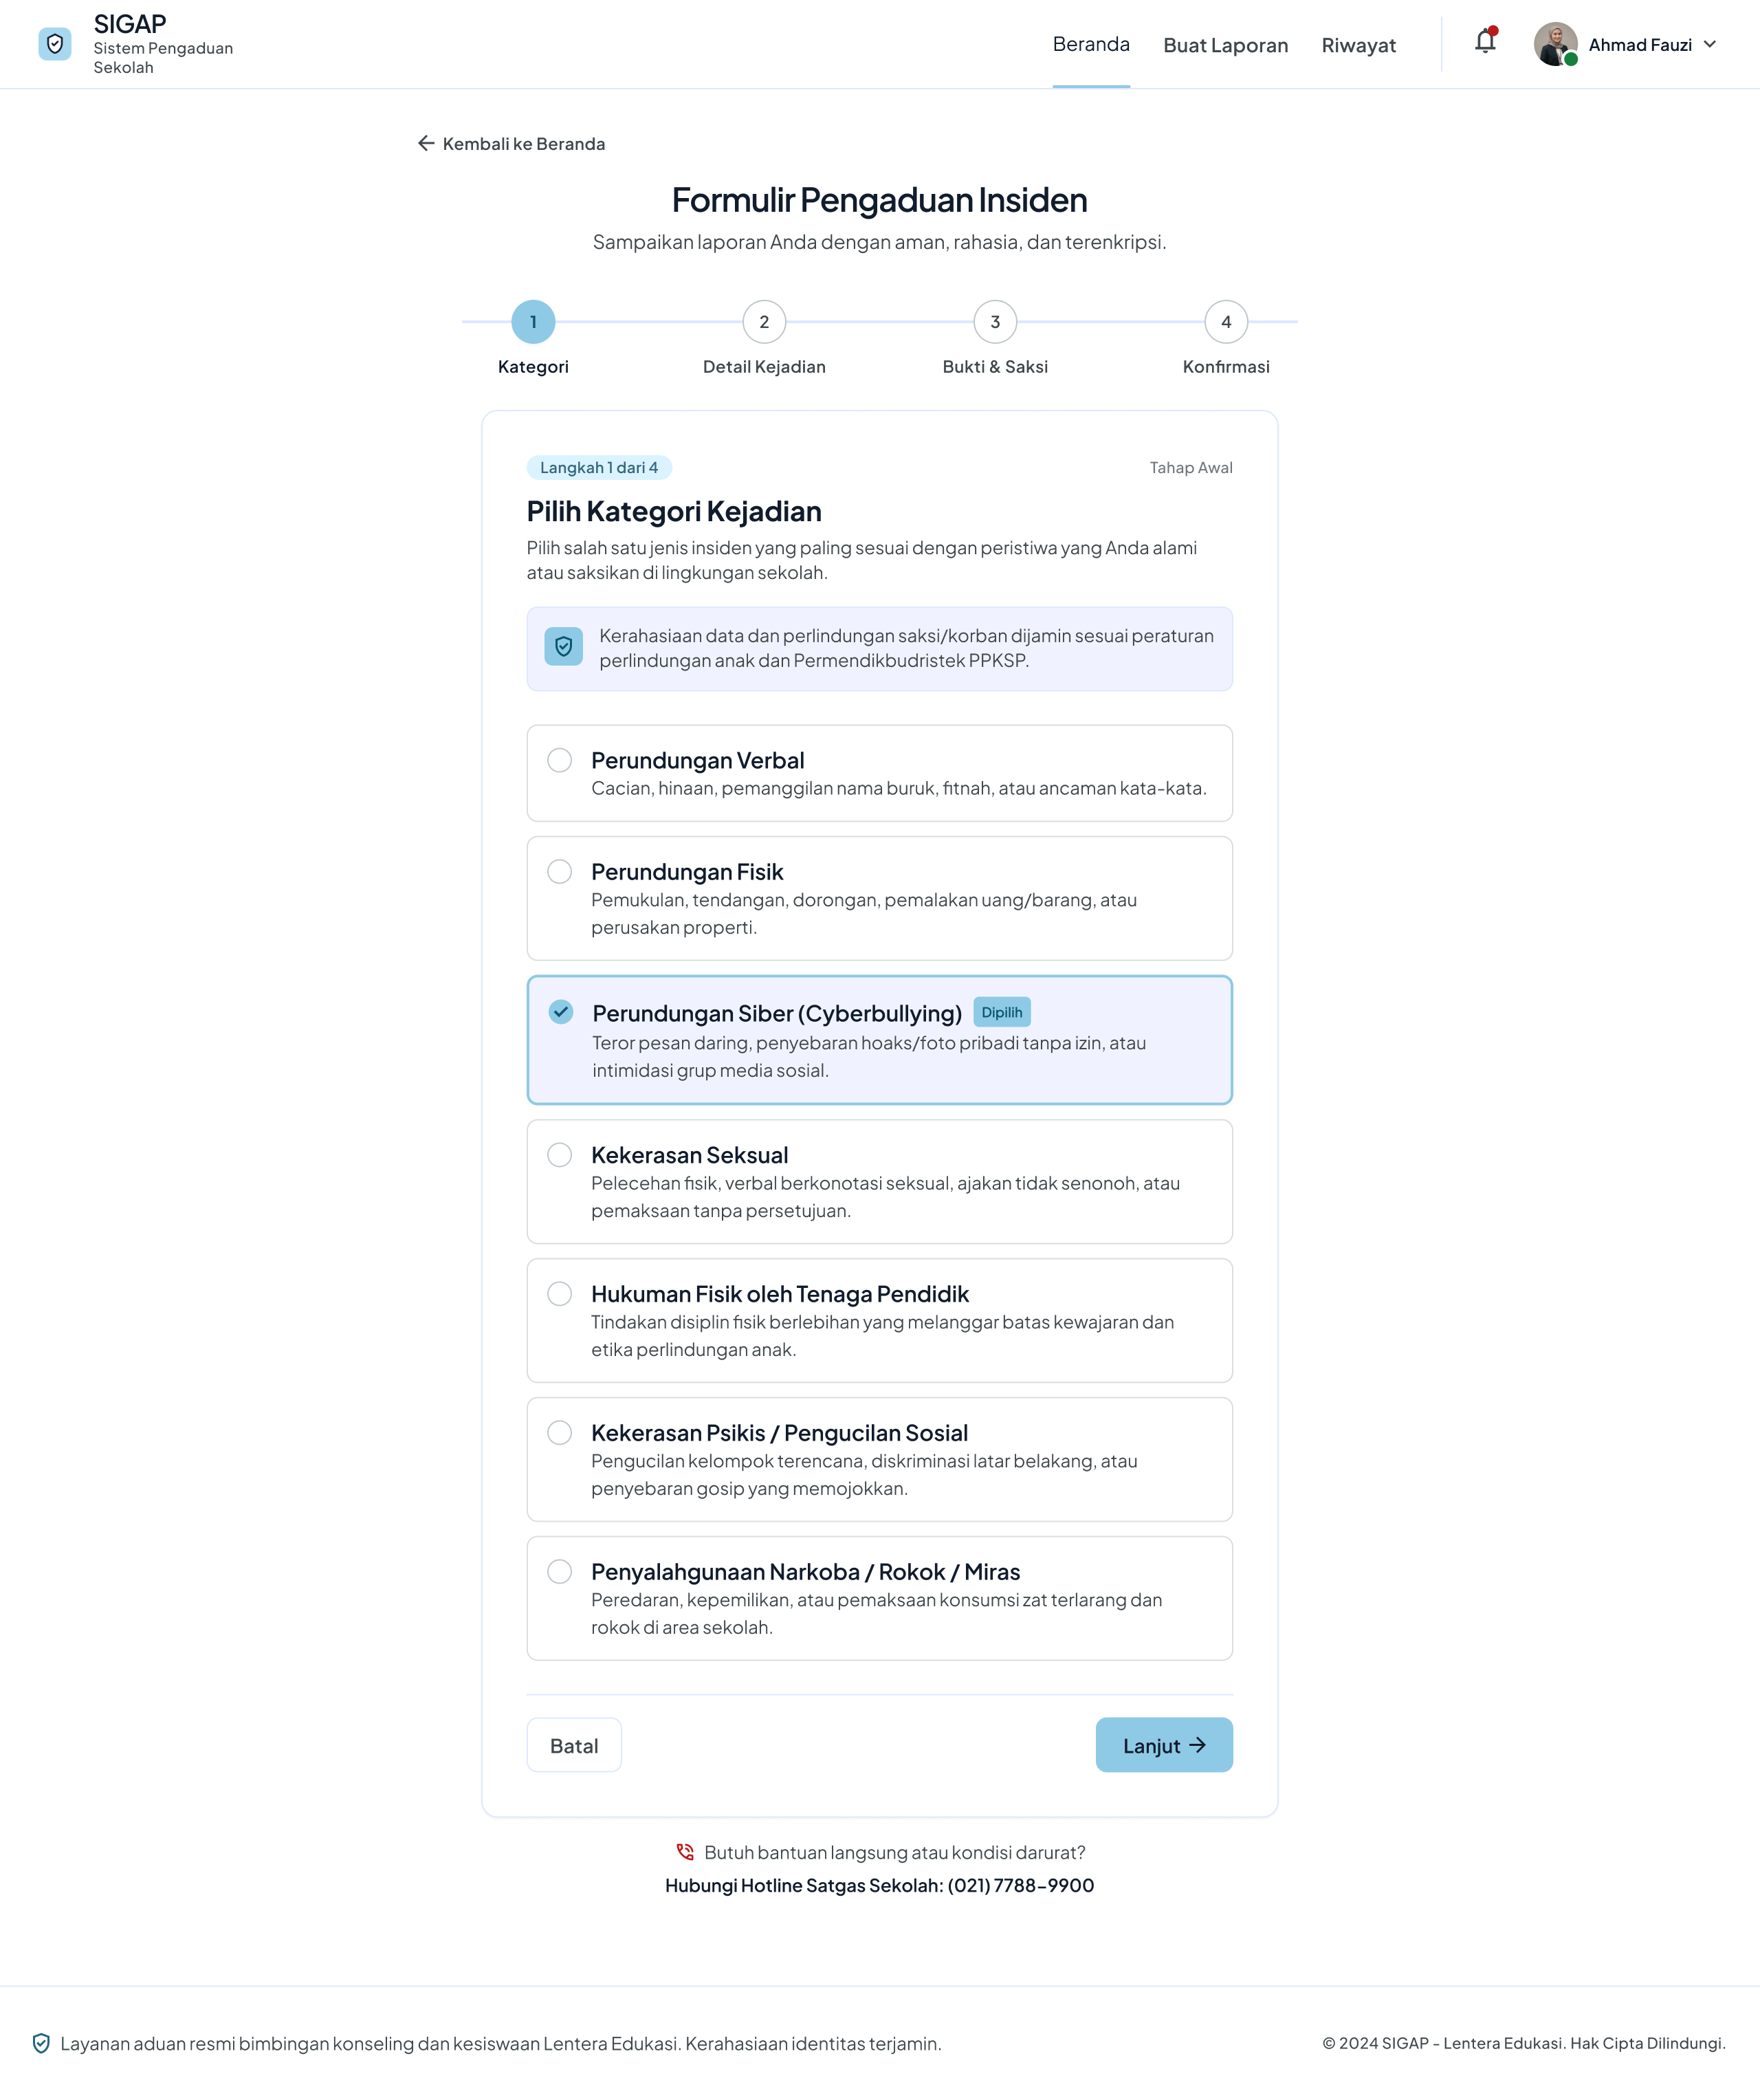
\includegraphics[width=\linewidth,height=0.42\textheight,keepaspectratio]{Frontend_image/FormulirPengaduanUser_SIGAP.png}
	\captionof{figure}{Formulir pengaduan pengguna siswa}
\end{minipage}
\hfill
\begin{minipage}[t]{0.48\linewidth}
	\centering
	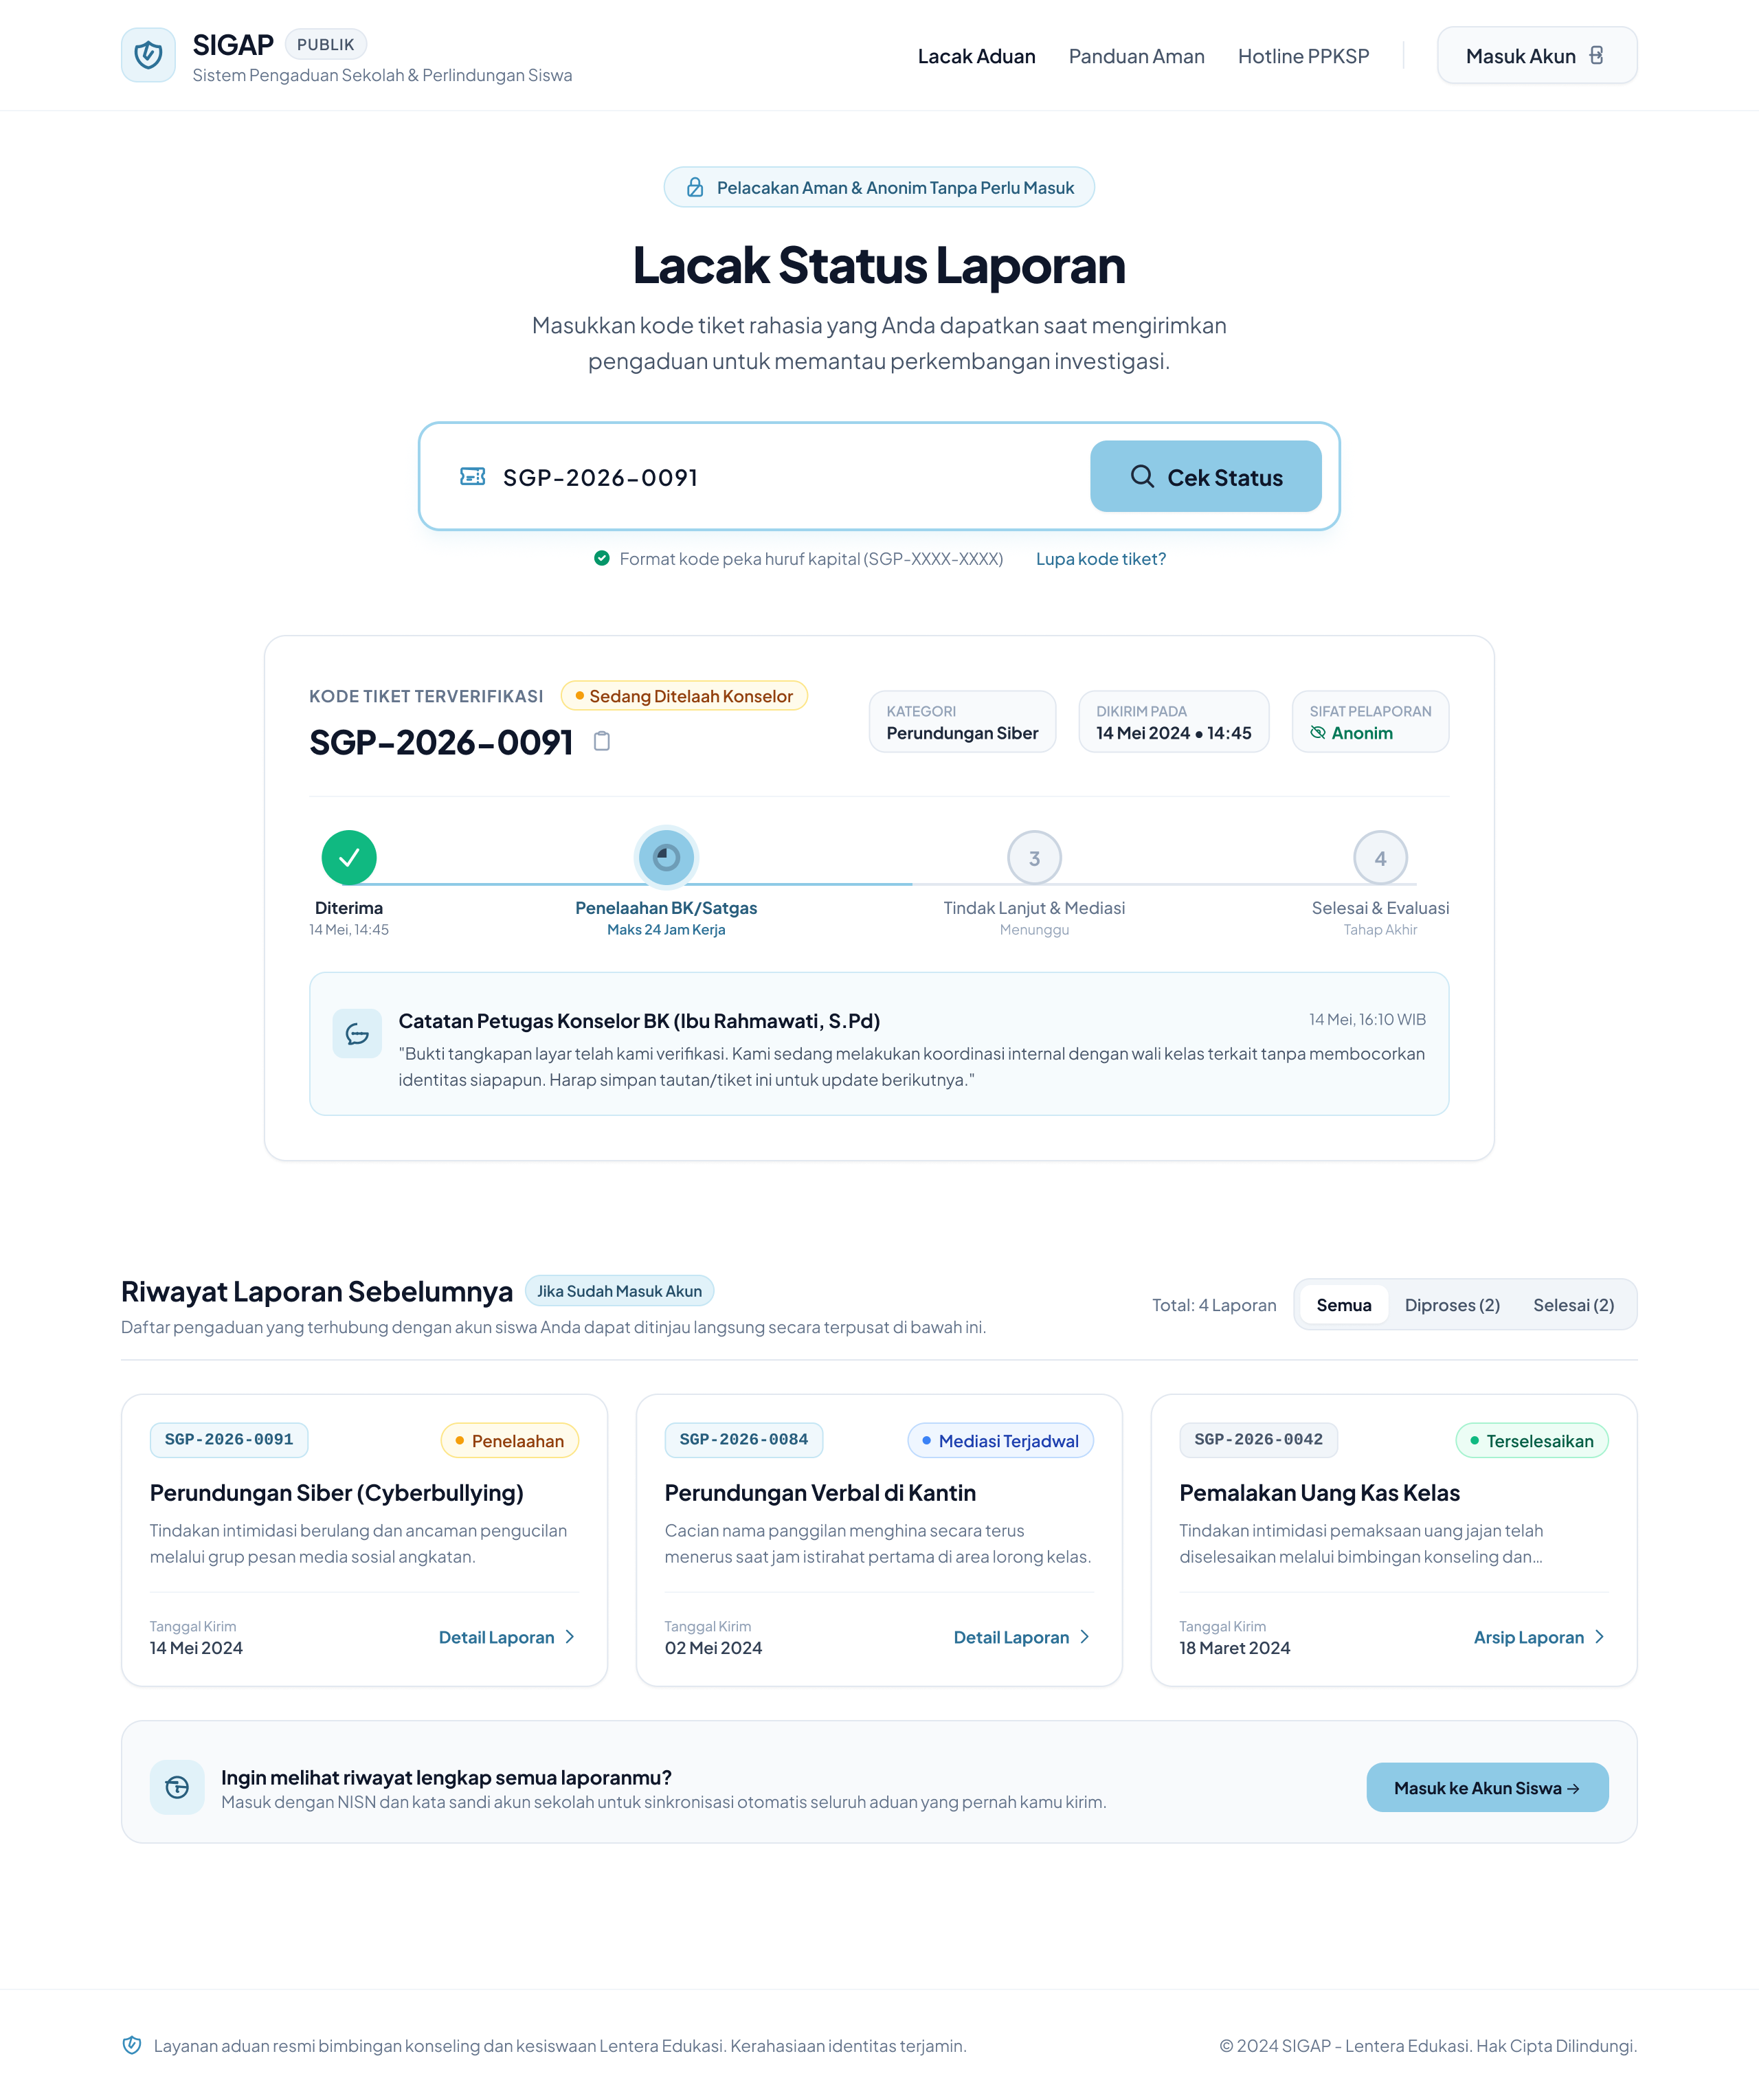
\includegraphics[width=\linewidth,height=0.42\textheight,keepaspectratio]{Frontend_image/LacakStatusLaporanUser_SIGAP.png}
	\captionof{figure}{Pelacakan status laporan pengguna siswa}
\end{minipage}

\vspace{0.8cm}
\noindent
\begin{minipage}[t]{0.48\linewidth}
	\centering
	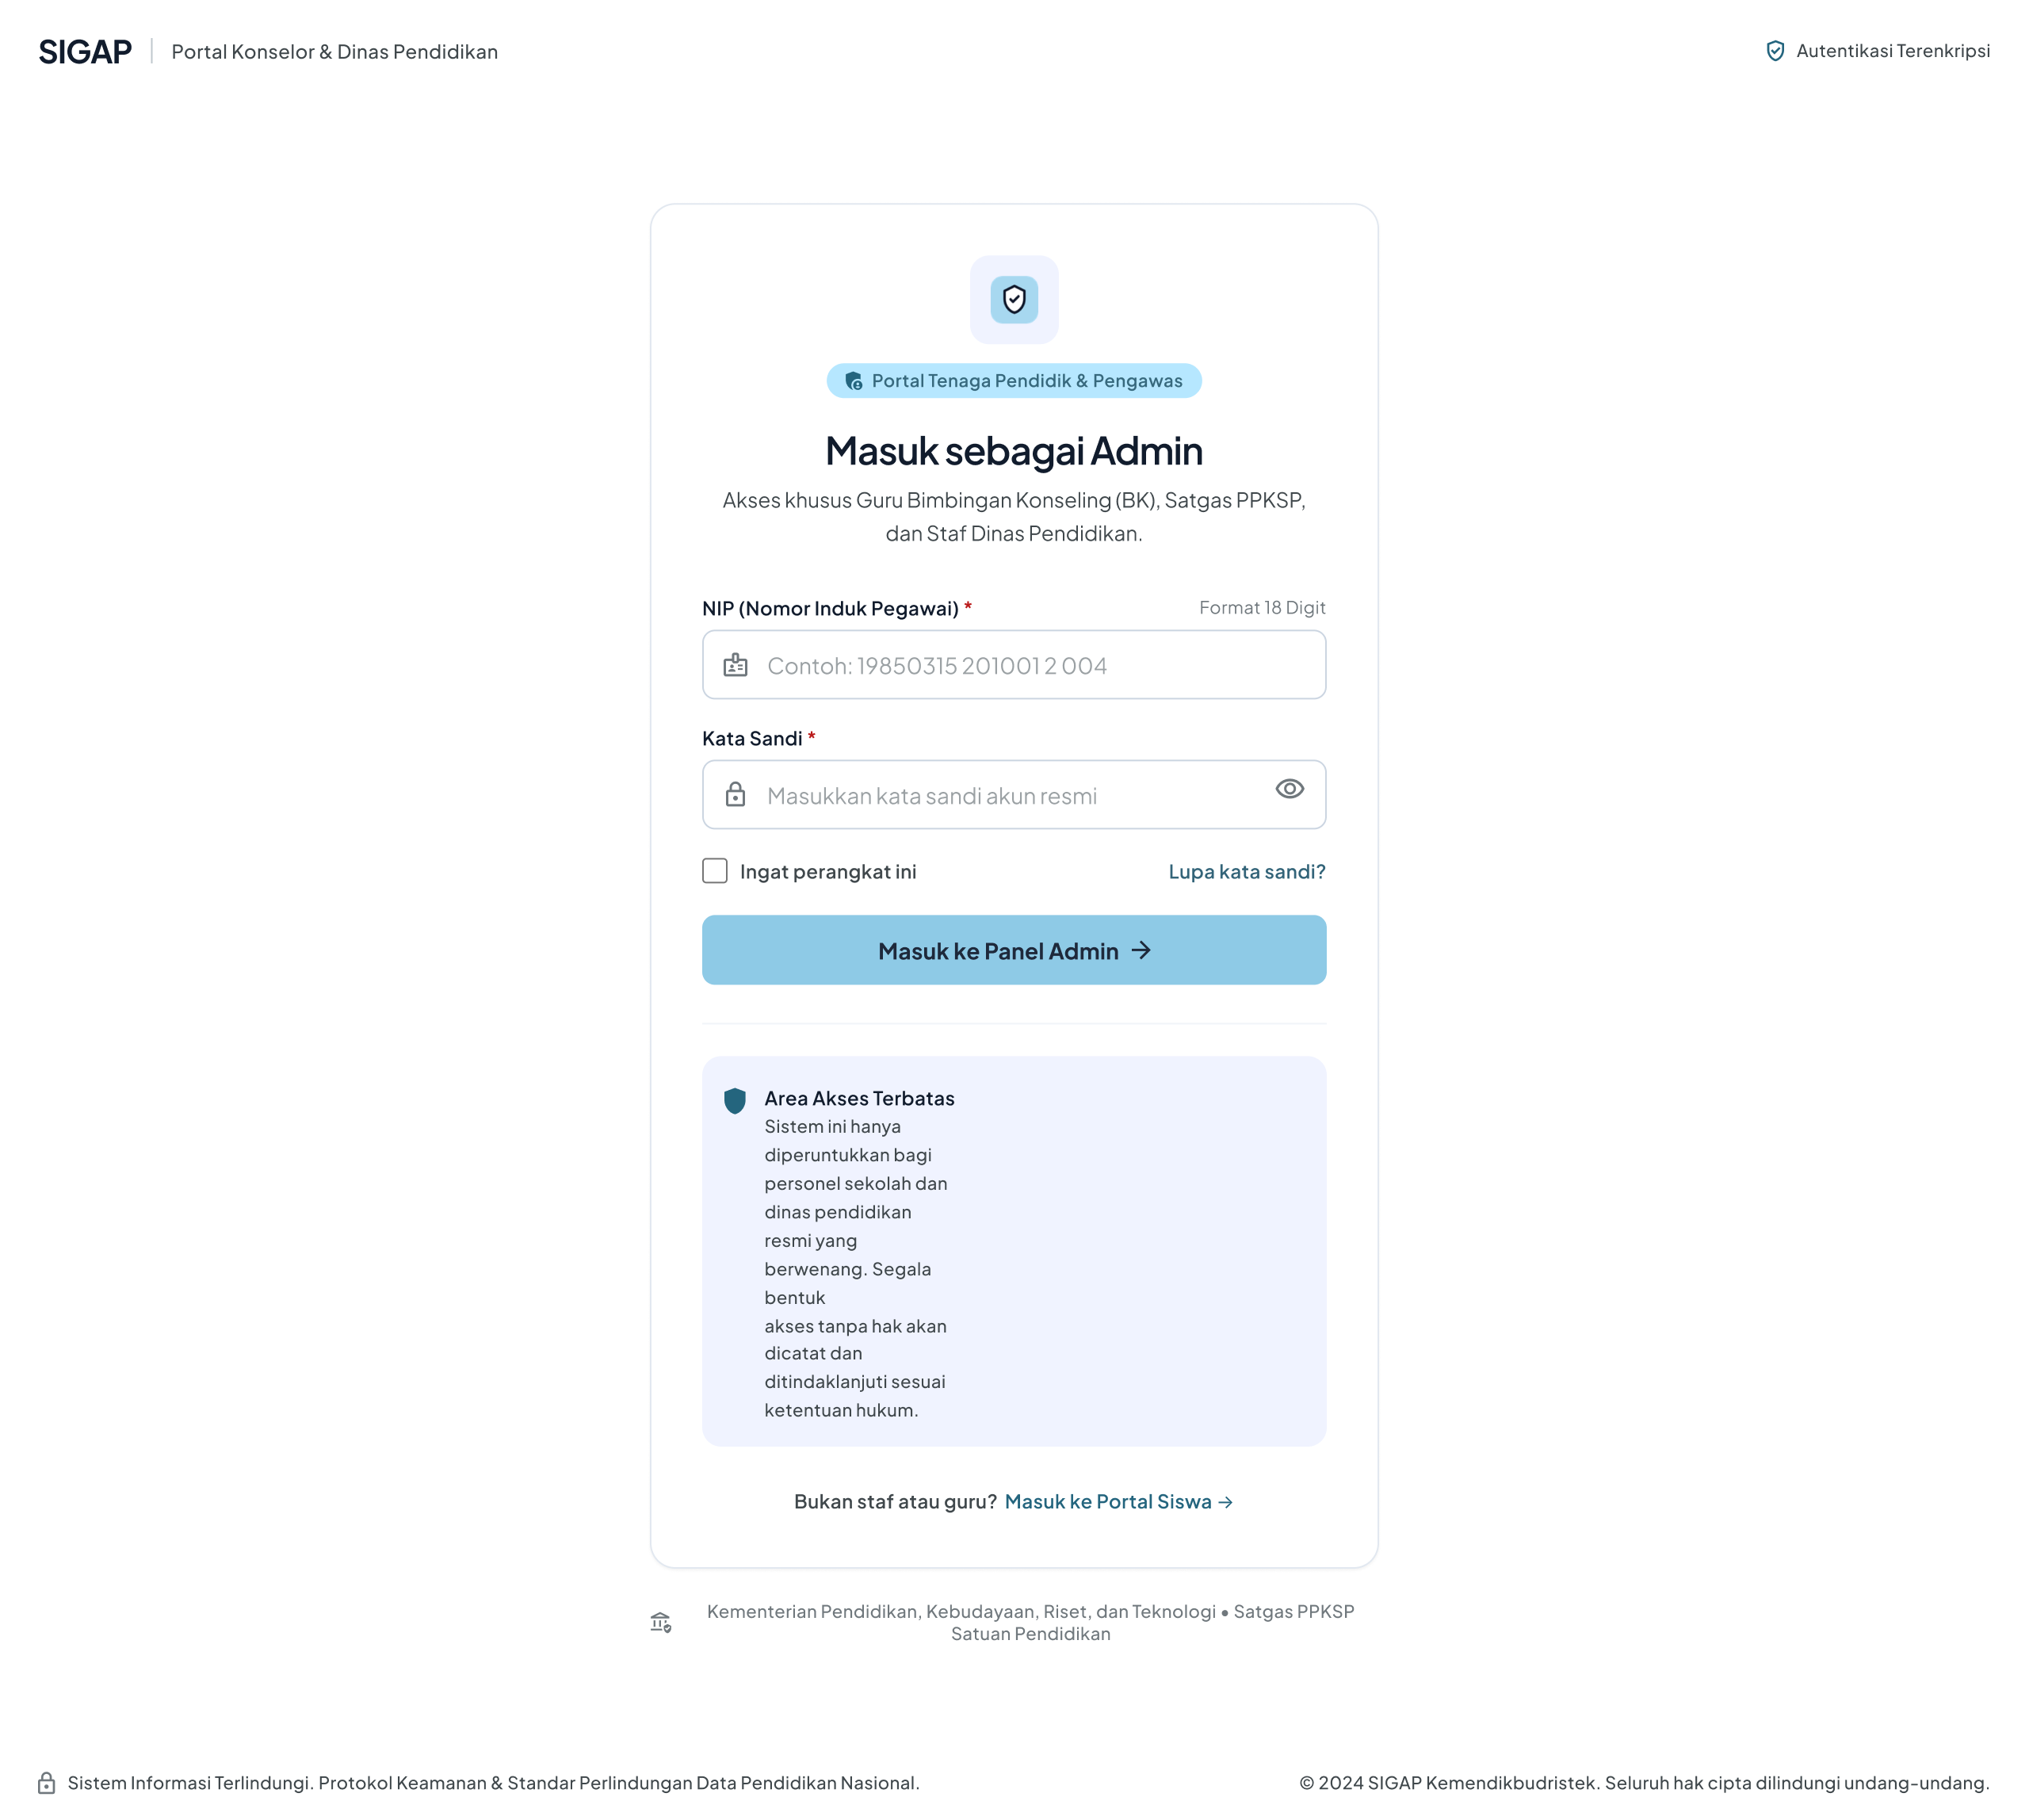
\includegraphics[width=\linewidth,height=0.42\textheight,keepaspectratio]{Frontend_image/OnBoardingAdmin_SIGAP.png}
	\captionof{figure}{Onboarding admin}
\end{minipage}
\hfill
\begin{minipage}[t]{0.48\linewidth}
	\centering
	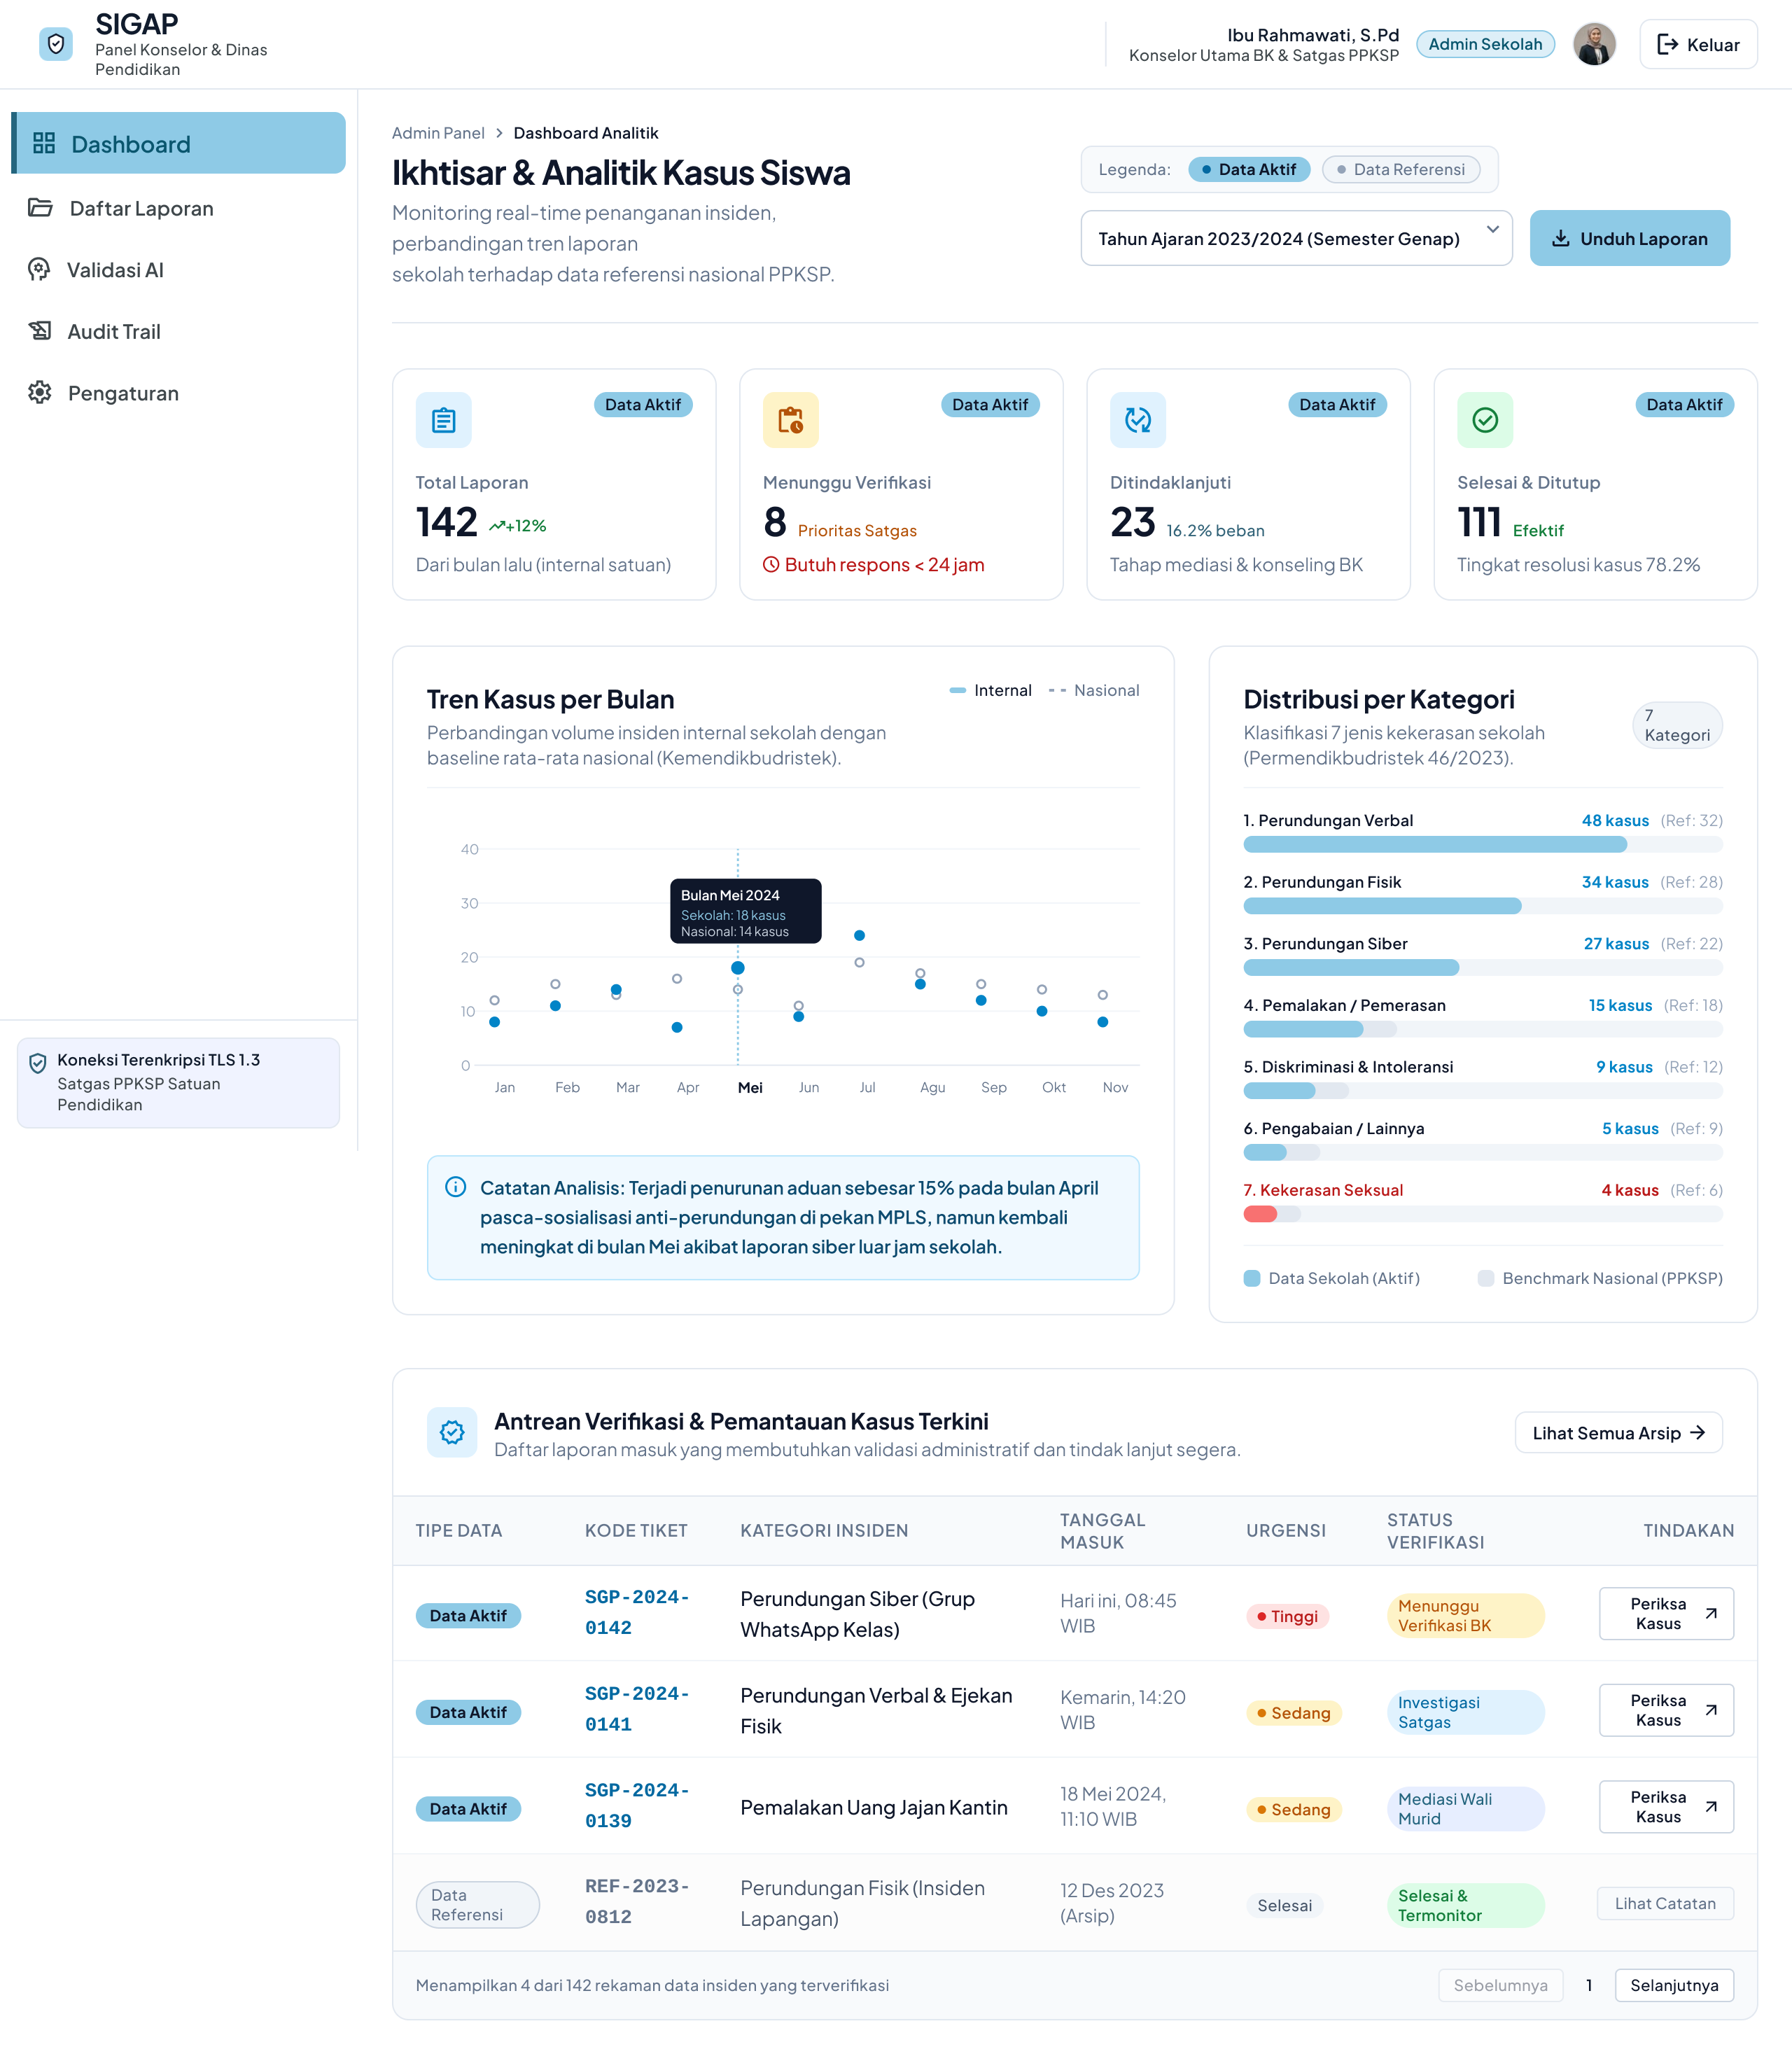
\includegraphics[width=\linewidth,height=0.42\textheight,keepaspectratio]{Frontend_image/DashboardAdmin_SIGAP.png}
	\captionof{figure}{Dashboard admin}
\end{minipage}

\vspace{0.8cm}
\noindent
\begin{minipage}[t]{0.48\linewidth}
	\centering
	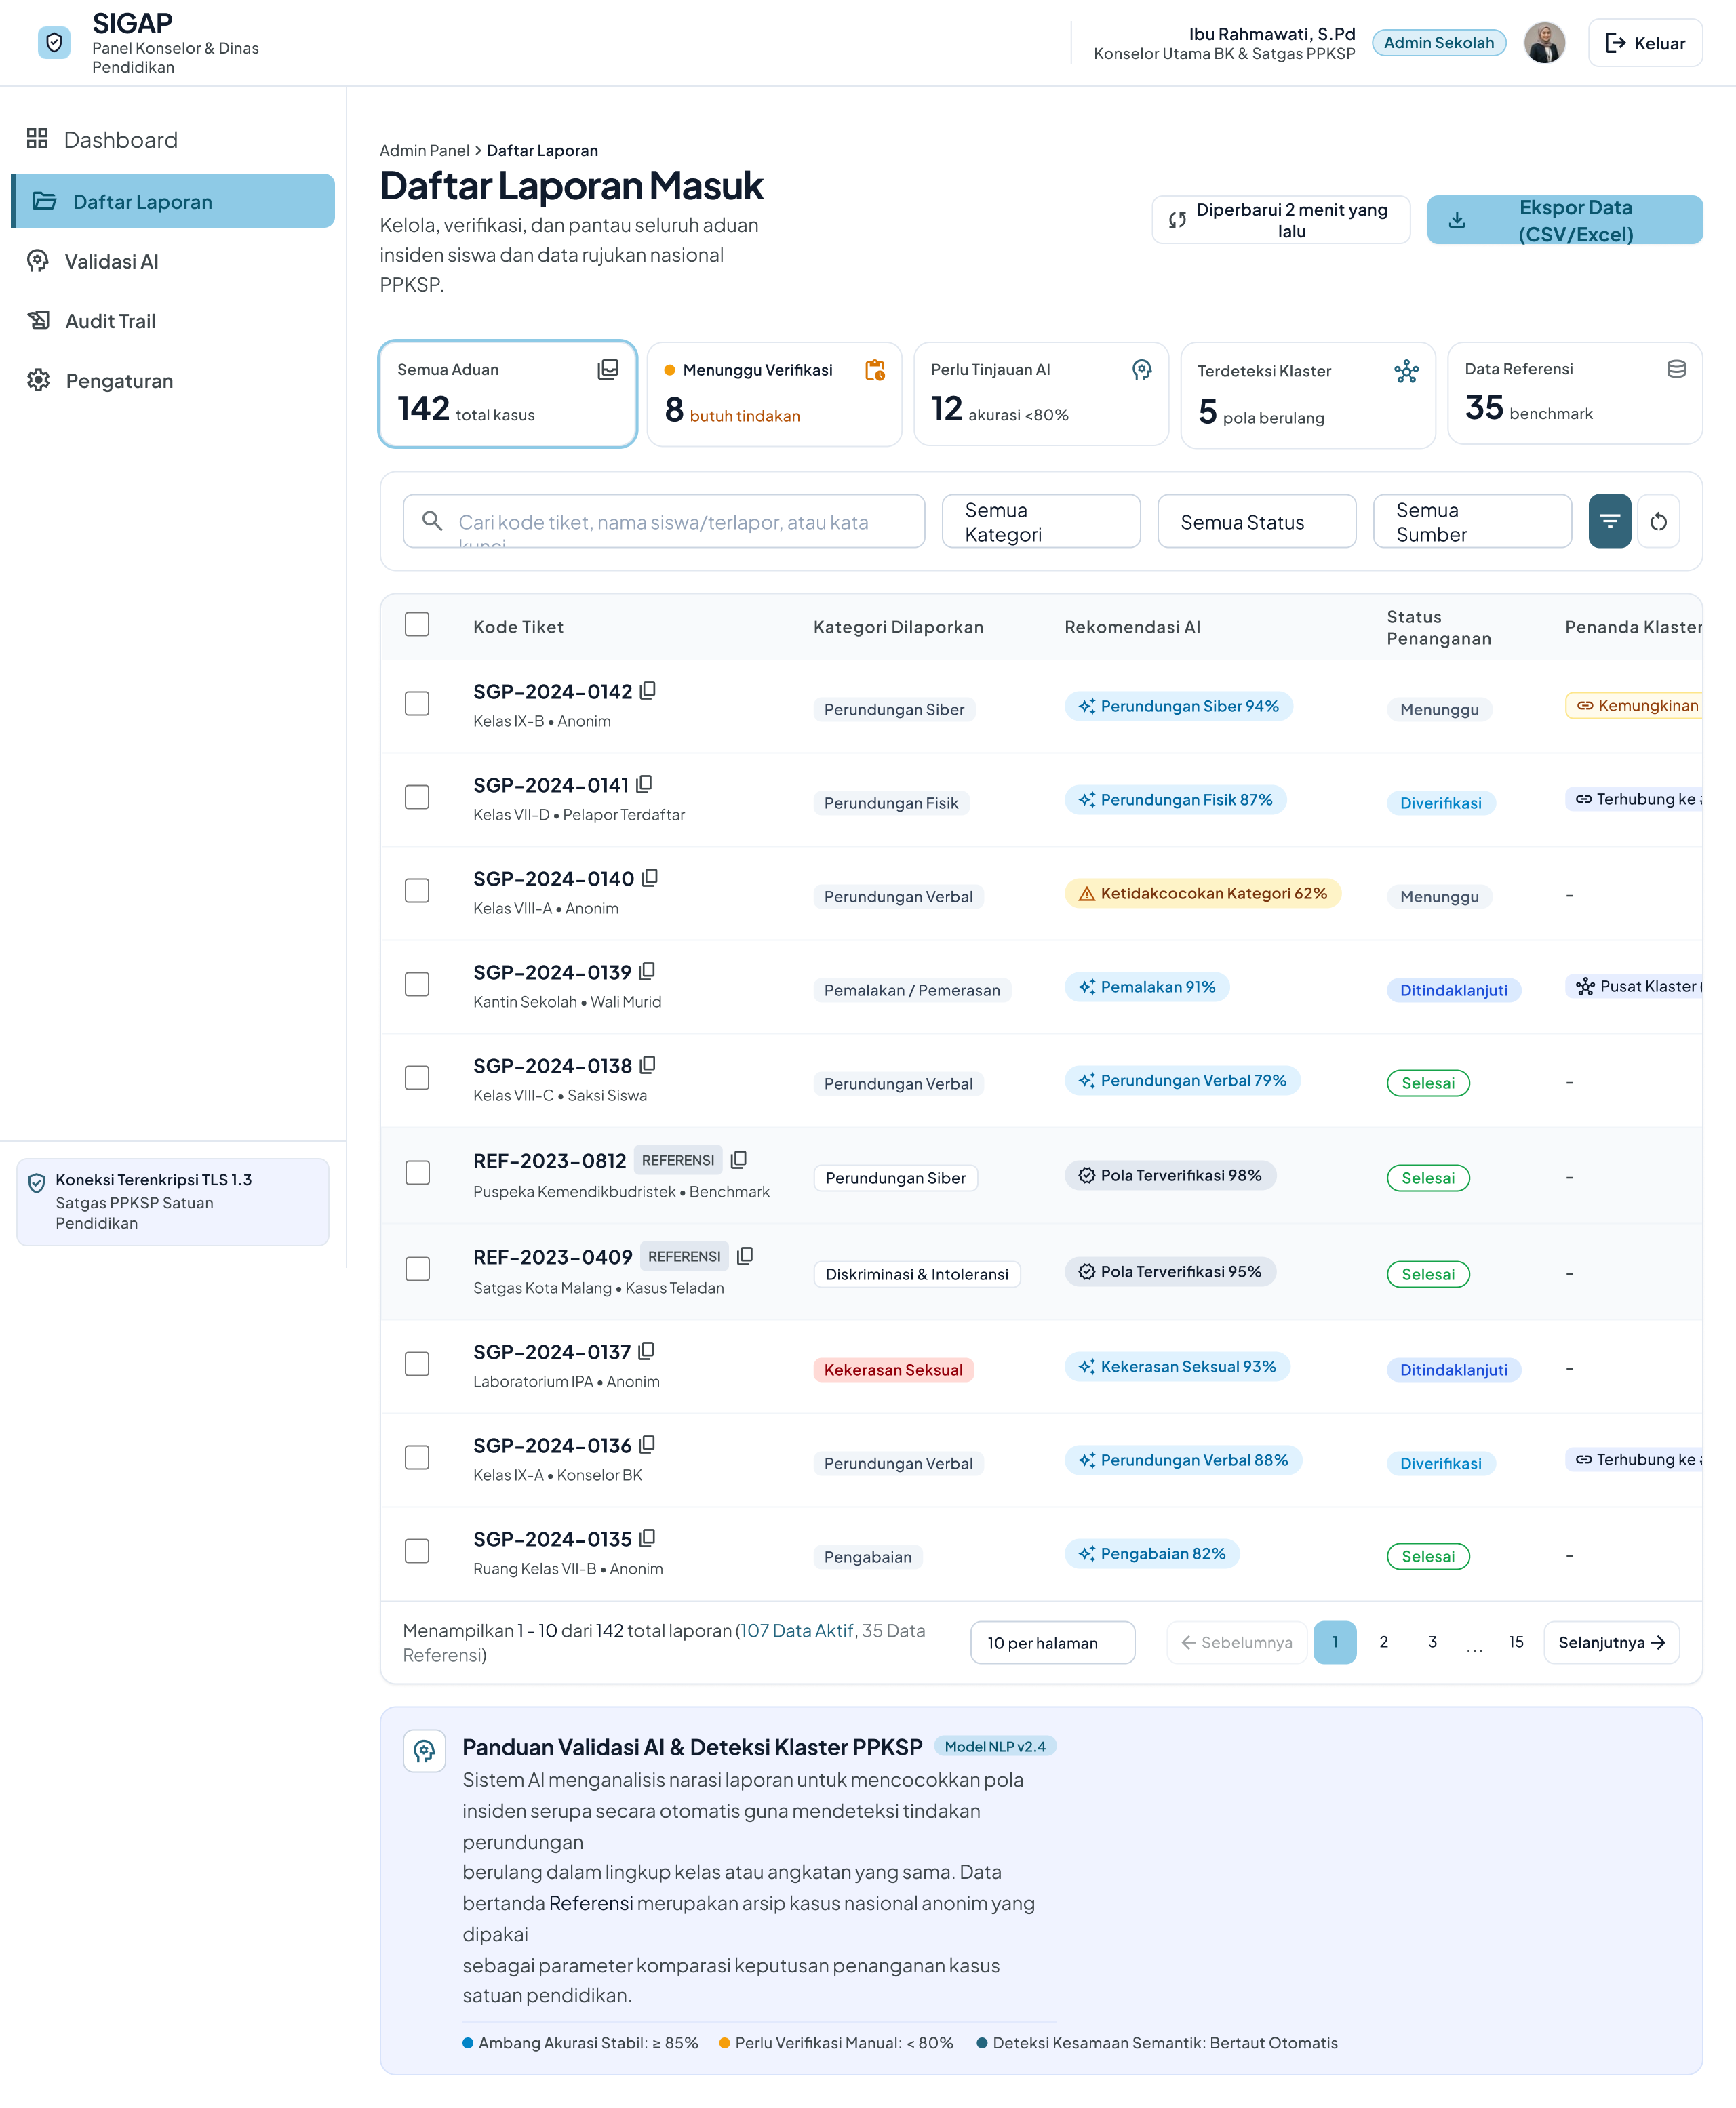
\includegraphics[width=\linewidth,height=0.42\textheight,keepaspectratio]{Frontend_image/DaftarLaporanMasukAdmin_SIGAP.png}
	\captionof{figure}{Daftar laporan masuk admin}
\end{minipage}
\hfill
\begin{minipage}[t]{0.48\linewidth}
	\centering
	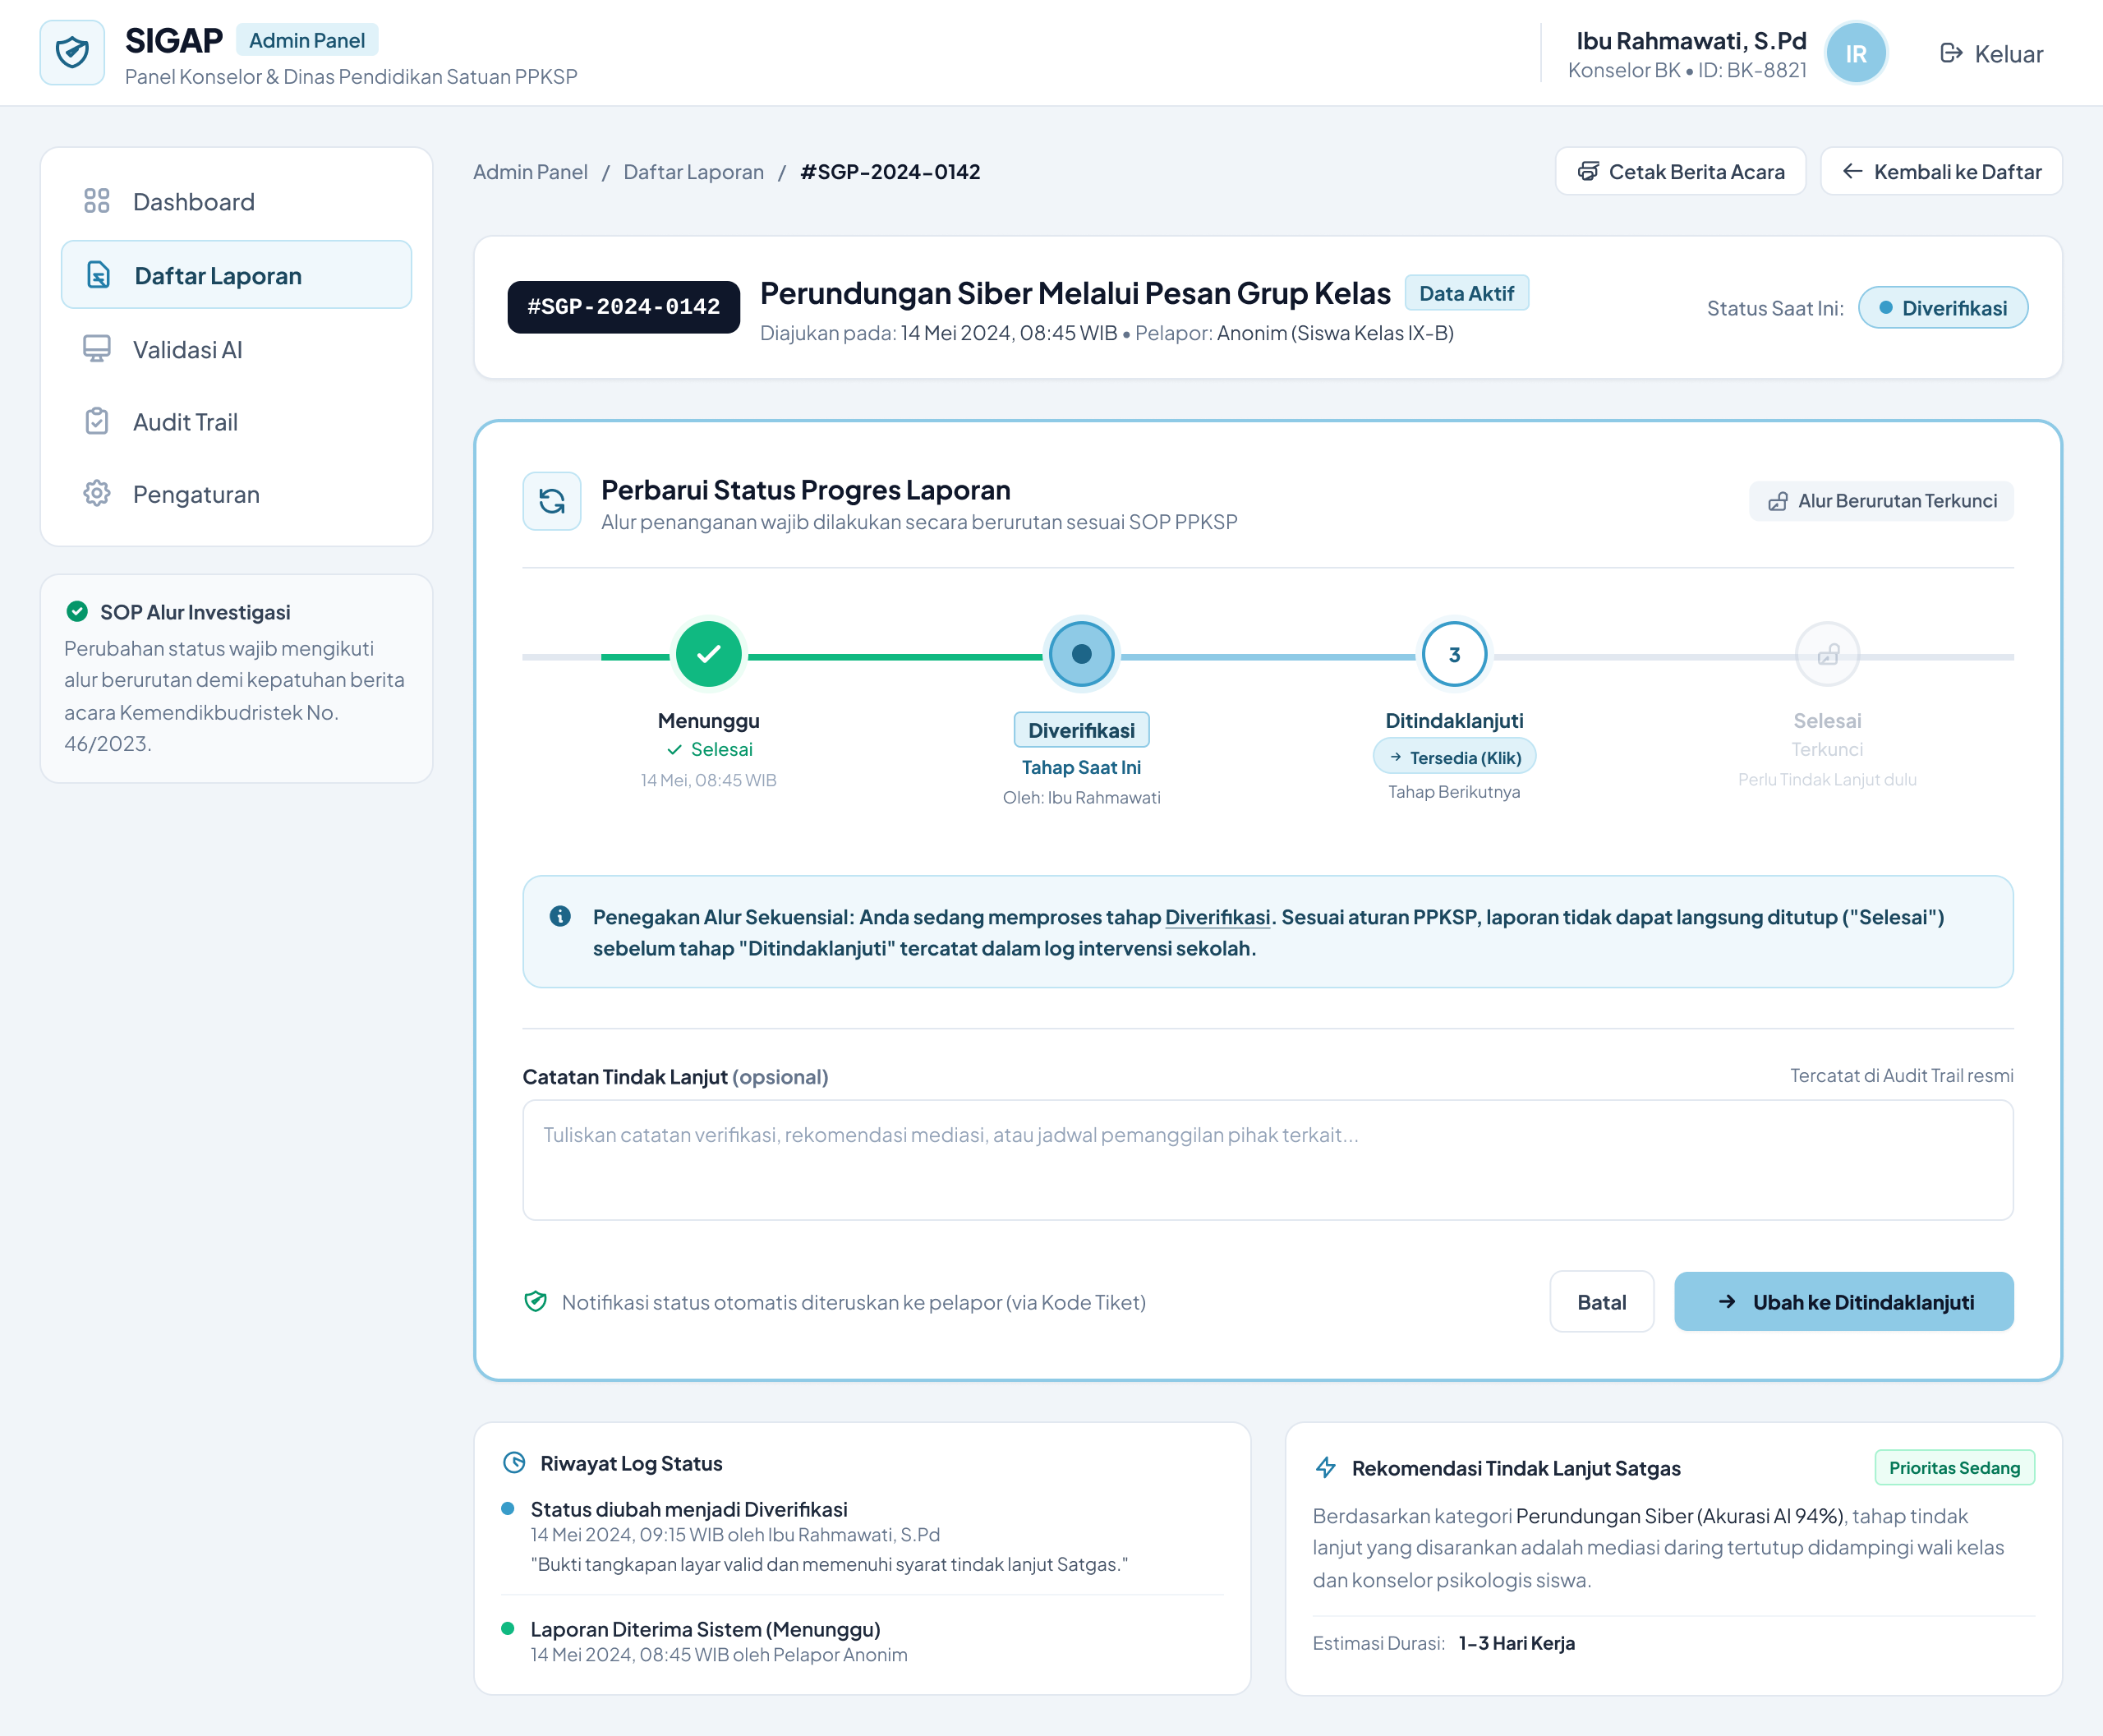
\includegraphics[width=\linewidth,height=0.42\textheight,keepaspectratio]{Frontend_image/StatusLaporanAdmin_SIGAP.png}
	\captionof{figure}{Status laporan pada sisi admin}
\end{minipage}

\vspace{0.8cm}
\noindent
\begin{minipage}[t]{0.48\linewidth}
	\centering
	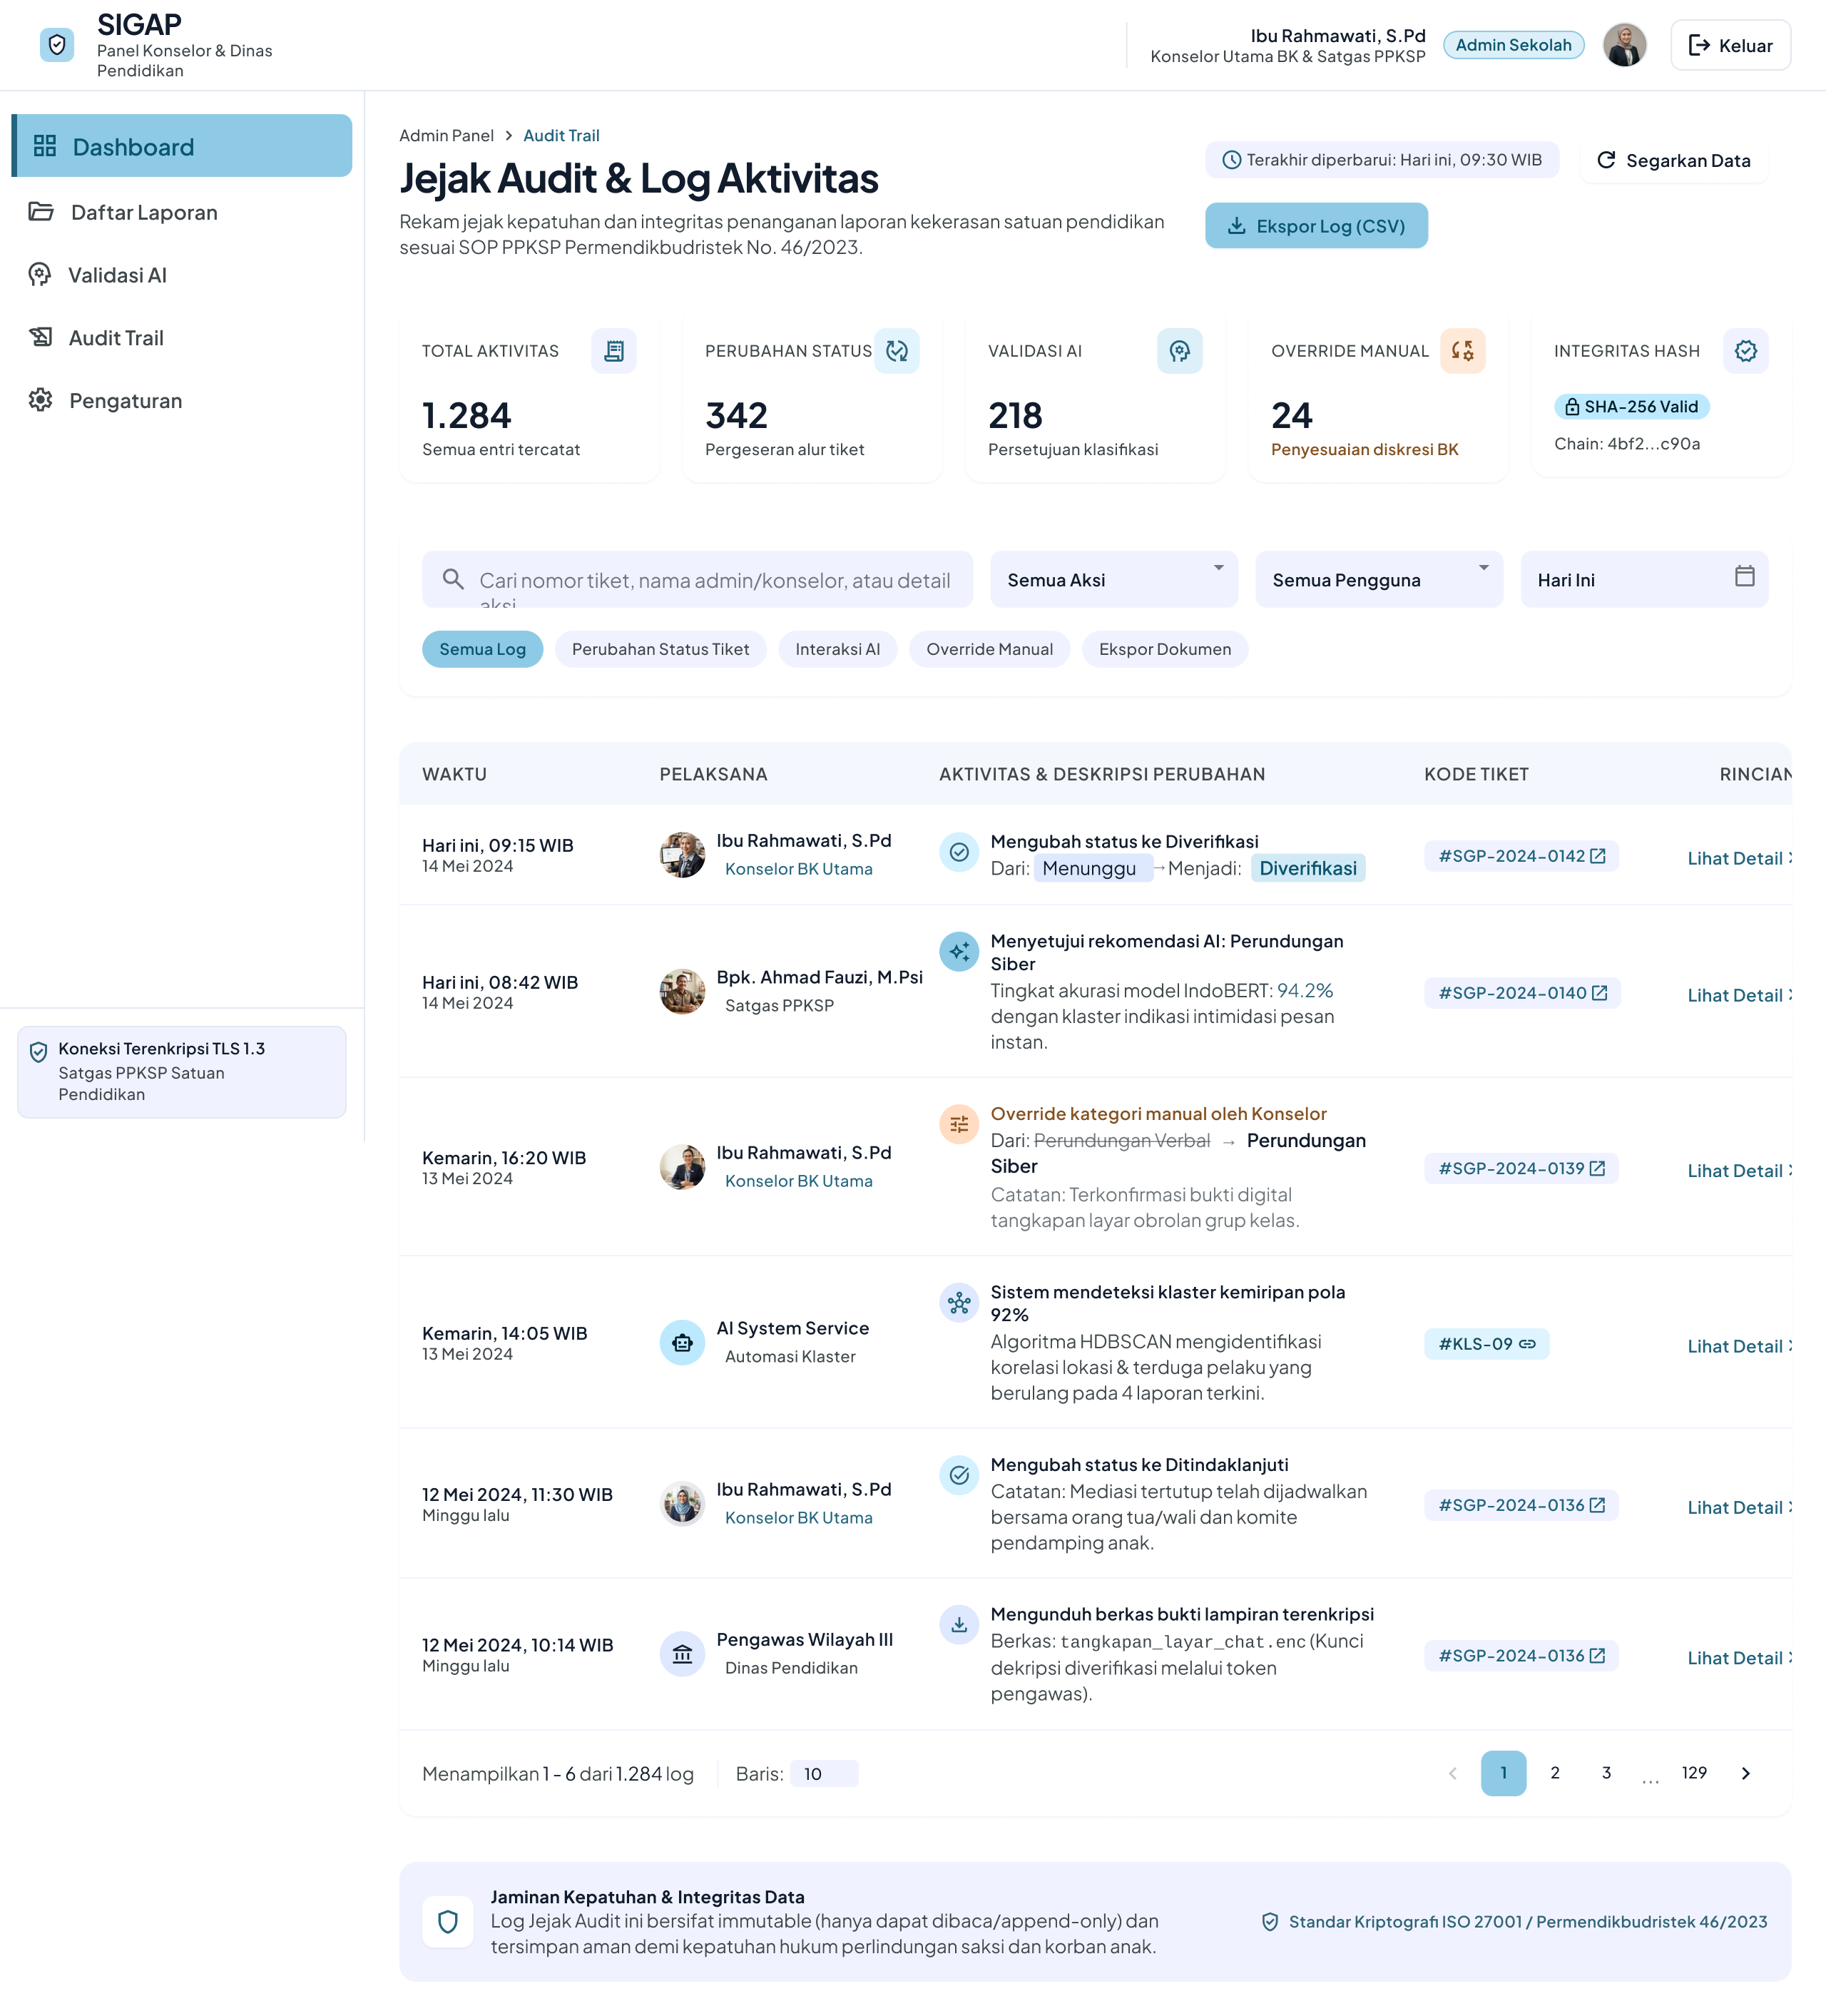
\includegraphics[width=\linewidth,height=0.42\textheight,keepaspectratio]{Frontend_image/JejakAuditAdmin_SIGAP.png}
	\captionof{figure}{Jejak audit admin}
\end{minipage}

\end{document}